\documentclass{aomart}

\usepackage[T1]{fontenc}
\usepackage[nopatch=footnote]{microtype}
\usepackage{amssymb,mathtools}
\usepackage{amscd}
\usepackage{bm}
\usepackage{aliascnt}
\usepackage{enumitem}
\usepackage{graphicx}
\usepackage{booktabs}
\usepackage{array}
\usepackage{longtable}
\usepackage[nameinlink,noabbrev]{cleveref}

\allowdisplaybreaks
\hyphenpenalty=10000
\exhyphenpenalty=10000
\tolerance=2600
\emergencystretch=4em

\makeatletter
\def\@setsubjects{%
  \let\@subjects\@empty
  \ifx\@primarysubjects\@empty\else
    \edef\@subjects{Primary:~\@primarysubjects}%
  \fi
  \ifx\@secondarysubjects\@empty\else
    \ifx\@primarysubjects\@empty
      \edef\@subjects{Secondary:~\@secondarysubjects}%
    \else
      \edef\@subjects{\@subjects, Secondary:~\@secondarysubjects}%
    \fi
  \fi
  \ifpdf
    \hypersetup{pdfsubject=\@subjects}%
  \fi
  \if@aom@oldkeywords\else
    \@footnotetext{AMS Classification:~\@subjects.}%
  \fi
}
\makeatother

\setlist[enumerate]{topsep=4pt,itemsep=2pt}
\setlist[itemize]{topsep=4pt,itemsep=2pt}

\newtheorem{theorem}{Theorem}[section]
\newaliascnt{proposition}{theorem}
\newtheorem{proposition}[proposition]{Proposition}
\aliascntresetthe{proposition}
\newaliascnt{lemma}{theorem}
\newtheorem{lemma}[lemma]{Lemma}
\aliascntresetthe{lemma}
\newaliascnt{corollary}{theorem}
\newtheorem{corollary}[corollary]{Corollary}
\aliascntresetthe{corollary}
\theoremstyle{definition}
\newaliascnt{definition}{theorem}
\newtheorem{definition}[definition]{Definition}
\aliascntresetthe{definition}
\newaliascnt{example}{theorem}
\newtheorem{example}[example]{Example}
\aliascntresetthe{example}
\newaliascnt{standardfact}{theorem}
\newtheorem{standardfact}[standardfact]{Standard Fact}
\aliascntresetthe{standardfact}
\theoremstyle{remark}
\newaliascnt{remark}{theorem}
\newtheorem{remark}[remark]{Remark}
\aliascntresetthe{remark}

\crefname{theorem}{theorem}{theorems}
\crefname{proposition}{proposition}{propositions}
\crefname{lemma}{lemma}{lemmas}
\crefname{corollary}{corollary}{corollaries}
\crefname{definition}{definition}{definitions}
\crefname{example}{example}{examples}
\crefname{standardfact}{standard fact}{standard facts}
\crefname{remark}{remark}{remarks}

\newcommand{\OO}{\mathcal O}
\newcommand{\FF}{\mathbb F}
\newcommand{\QQ}{\mathbb Q}
\newcommand{\ZZ}{\mathbb Z}
\newcommand{\CC}{\mathbb C}
\newcommand{\NN}{\mathbb N}
\newcommand{\Spec}{\operatorname{Spec}}
\newcommand{\Spf}{\operatorname{Spf}}
\newcommand{\Supp}{\operatorname{Supp}}
\newcommand{\Ann}{\operatorname{Ann}}
\newcommand{\Fitt}{\operatorname{Fitt}}
\newcommand{\Hom}{\operatorname{Hom}}
\newcommand{\End}{\operatorname{End}}
\newcommand{\coker}{\operatorname{coker}}
\newcommand{\im}{\operatorname{im}}
\newcommand{\rank}{\operatorname{rank}}
\newcommand{\Tr}{\operatorname{Tr}}
\newcommand{\Frob}{\operatorname{Frob}}
\newcommand{\Gal}{\operatorname{Gal}}
\newcommand{\GL}{\operatorname{GL}}
\newcommand{\red}{\operatorname{red}}
\newcommand{\Def}{\operatorname{Def}}
\newcommand{\ad}{\operatorname{ad}}
\newcommand{\Ob}{\operatorname{Ob}}
\newcommand{\SCC}{\operatorname{SCC}}
\newcommand{\length}{\operatorname{length}}
\newcommand{\rad}{\operatorname{rad}}
\newcommand{\id}{\operatorname{id}}
\newcommand{\e}{\mathrm e}
\newcommand{\one}{\bm 1}
\newcommand{\norm}[1]{\left\lVert#1\right\rVert}
\newcommand{\abs}[1]{\left\lvert#1\right\rvert}
\newcommand{\calF}{\mathcal F}
\newcommand{\calX}{\mathcal X}
\newcommand{\calC}{\mathcal C}
\newcommand{\calM}{\mathcal M}
\newcommand{\calA}{\mathcal A}
\newcommand{\calP}{\mathcal P}
\newcommand{\calR}{\mathcal R}
\newcommand{\calS}{\mathcal S}
\newcommand{\calV}{\mathcal V}
\newcommand{\calW}{\mathcal W}
\newcommand{\mathfrakF}{\mathfrak F}
\newcommand{\mathfrakC}{\mathfrak C}
\newcommand{\mathfrakT}{\mathfrak T}

\graphicspath{{figures/}}

\title[Residual deformation forests]{Residual Deformation Forests, Companion Systems, and Module Support}
\author[Komorebi P.]{Komorebi P.}
\subject{primary}{msc2020}{11F80}
\subject{secondary}{msc2020}{13B35}
\subject{secondary}{msc2020}{13D10}
\subject{secondary}{msc2020}{11R34}
\subject{secondary}{msc2020}{14B12}
\keyword{Galois deformation}
\keyword{inverse limit}
\keyword{compatible system}
\keyword{Fitting ideal}
\keyword{module support}
\keyword{occupancy}
\copyrightnote{}
\doinumber{}

\pdfstringdefDisableCommands{\let\unskip\relax}
\hypersetup{
  pdftitle={Residual Deformation Forests, Companion Systems, and Module Support},
  pdfauthor={Komorebi P.},
  pdfsubject={Residual fibers, deformation levels, companion systems, finite Frobenius separation, module support, and occupancy}
}

\begin{document}
\begin{abstract}
Let \(\OO\) be a complete discrete valuation ring. A deformation problem over \(\OO\) separates into residual fibers, and every positive depth lift remains inside one such fiber. We study the resulting inverse systems of finite lift levels and give exact branch criteria based on the Mittag Leffler condition, finite branching, and completeness. Smooth, weighted, nilpotent, and normal crossing charts have explicit level counts and rational counting series. Compatible projectors split tangent and obstruction complexes, so a lift exists precisely when every packet obstruction vanishes. Horizontal transport is encoded by a directed category whose minimum number of residual generators is the number of source components. A common algebraic Frobenius spine turns local companion forests into one compatible system once every finite level is occupied. Finite Frobenius traces separate irreducible compatible constituents and recover their multiplicities inside a known carrier. The final part replaces finite spectral occupancy by module support. For a finite module, occupancy is detected by its zeroth Fitting ideal, behaves well under flat base change, and extends to nonsemisimple Artinian packets. We also give exact hypotheses under which nonvanishing survives infinitely many compatible conditions.
\end{abstract}
\maketitle
\thispagestyle{plain}

\section{Introduction}\label{sec:introduction}

A deformation problem has two directions that should not be merged. The first direction is vertical. One fixes a residual object and lifts it through successive powers of a maximal ideal. The second direction is horizontal. One changes the residual root, the coefficient prime, or the ambient arithmetic carrier. Deeper vertical precision does not create a missing horizontal companion.

The distinction is elementary at the first level. Let \(\OO\) be a complete discrete valuation ring with uniformizer \(\varpi\), residue field \(k\), and fraction field \(K\). If two integral objects differ by a correction divisible by \(\varpi\), then they have the same reduction in characteristic \(\operatorname{char}k\). A branch above one residual root can explore its entire formal neighborhood, but it cannot cross to another root. In the deformation theory of Galois representations, this is built into the usual deformation functor of a fixed residual representation \cite{Mazur1989,Ramakrishna1993,Kisin2010}. General representability questions are governed by Schlessinger's criteria \cite{Schlessinger1968}. Pseudorepresentations provide a broader residual moduli language when an ordinary representation functor is not available \cite{Chenevier2014,BellaicheChenevier2009}.

The first part of the article studies a residual fiber as an inverse system
\[
X_1\longleftarrow X_2\longleftarrow X_3\longleftarrow\cdots.
\]
A complete lift is a compatible branch. Represented deformation problems reconstruct their \(\OO\) valued points from this inverse limit. Finite branching gives a second existence mechanism through K\"onig's lemma. The more flexible condition is the Mittag Leffler condition. It allows dead branches at finite depth while retaining a stable nonempty core.

The number of points at level \(m\) records local geometry. The valuation conventions used below are standard for complete discrete valuation rings and local fields \cite{Serre1979}. A smooth formal chart of relative dimension \(d\) has \(q^{d(m-1)}\) points above a fixed residual root. Weighted coordinates delay the first visible digit. Nilpotent charts and normal crossings have different growth laws. We derive their counting series directly. These formulas are elementary special cases of a much broader rationality theory for local counting series \cite{Denef1984}. They are included because their exact exponents later measure branch growth and delayed visibility.

The second part concerns tangent and obstruction spaces. Galois deformation theory identifies tangent directions with first cohomology and places obstructions in second cohomology under the standard hypotheses \cite{Mazur1989,NeukirchSchmidtWingberg2008}. If a finite family of chain projectors commutes with the differential, the full correction complex splits into subcomplexes. We use the standard language of cochain complexes and cohomology \cite{Weibel1994}. Tangent directions and obstruction classes then split packet by packet. This gives an exact criterion. A lift exists if and only if every packet obstruction vanishes.

Horizontal transport is treated separately. A directed edge between residual roots means that a declared arithmetic operation carries one residual problem into another while preserving the chosen local conditions. For a finite transport graph, the minimum number of residual starting points is the number of source strongly connected components. This is a graph theorem, not a companion existence theorem. The graph can describe how existing roots generate one another, but it cannot supply a missing vertex.

A compatible system requires one algebraic spine. We use Frobenius characteristic polynomials and selected local labels as the common data. At each coefficient place \(\lambda\), the finite companion sets form a lift forest. If the stable images are nonempty at every depth, each local forest has a branch. The product of the local branch spaces then gives a simultaneous family. The conclusion is conditional on the nonemptiness of every companion forest. It does not prove that residual companions exist.

The last part changes the meaning of occupancy. In a fixed finite dimensional semisimple carrier over a field of characteristic zero, a joint spectral packet is occupied exactly when its projector has positive rank, equivalently nonzero trace. That criterion is exact, but it depends on semisimplicity and on a carrier chosen in advance. A deformation ring or a Hecke algebra is usually not semisimple. The natural replacement is the support of a finite module over a commutative ring. We prove
\[
\Supp_R(M)
=
V\bigl(\Fitt_0^R(M)\bigr)
=
V\bigl(\Ann_R(M)\bigr).
\]
The zeroth Fitting ideal therefore detects occupancy by explicit minors of a presentation matrix. Central idempotents recover the finite packet picture, while local support and completion handle nonsemisimple components.

There is one further distinction. Nonvanishing at every finite stage need not imply nonvanishing after infinitely many conditions. In finite dimension, a descending chain stabilizes. In an infinite dimensional space it may collapse to zero. We state exact positive criteria based on finite length, compactness, the Mittag Leffler property, and adic completeness.

\begin{figure}[t]
\centering
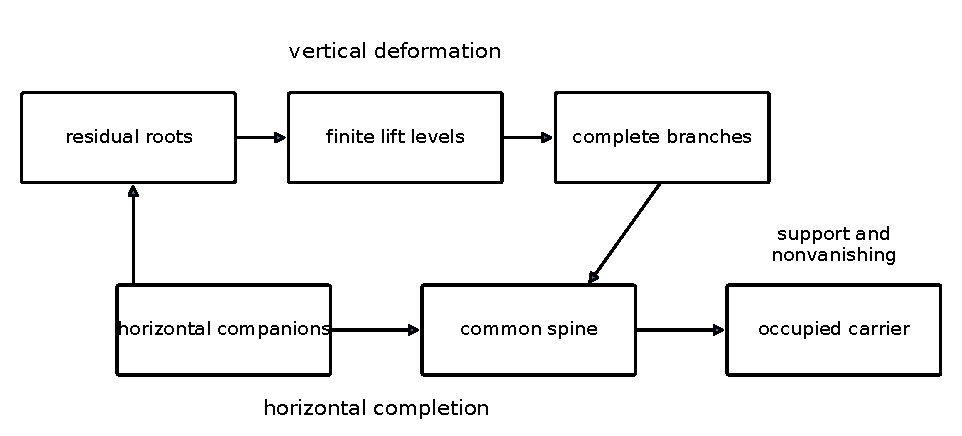
\includegraphics[width=.98\textwidth]{01_architecture.pdf}
\caption{Vertical lifting, horizontal companion formation, and support occupancy are separate operations. The final conclusion needs all three.}
\label{fig:architecture}
\end{figure}

The main results are arranged as follows. Residual fibers and inverse limits appear in \cref{sec:residual}. Visibility filtrations and counting series are treated in \cref{sec:counting}. Deformation complexes and packet obstructions appear in \cref{sec:obstruction}. Residual transport is studied in \cref{sec:transport}. Companion systems and finite Frobenius separation are developed in \cref{sec:companions,sec:frobenius}. Support occupancy and its finite dimensional specialization appear in \cref{sec:support,sec:finiteoccupancy}. Infinite occupancy and the conditional completion theorem close the article.

\section{Residual fibers and lift forests}\label{sec:residual}

\subsection{Coefficient rings and residual fibers}

Let \(\OO\) be a complete discrete valuation ring with maximal ideal \((\varpi)\), residue field
\[
k=\OO/(\varpi),
\qquad
\abs{k}=q,
\]
and fraction field \(K\). Let \(\mathsf C_{\OO}\) denote a category of complete local Noetherian \(\OO\) algebras with residue field \(k\). Let
\[
\calM:\mathsf C_{\OO}\longrightarrow\mathsf{Sets}
\]
be a functor equipped with natural reduction maps
\[
\red_A:\calM(A)\longrightarrow\calM(k).
\]

\begin{definition}[Residual fiber]\label{def:residual_fiber}
For \(\bar x\in\calM(k)\), define
\[
\calM_{\bar x}(A)
=
\{x\in\calM(A):\red_A(x)=\bar x\}.
\]
The point \(\bar x\) is the residual root of every object in this fiber.
\end{definition}

\begin{proposition}[Residual partition]\label{prop:residual_partition}
For every \(A\in\mathsf C_{\OO}\),
\[
\boxed{
\calM(A)
=
\bigsqcup_{\bar x\in\calM(k)}
\calM_{\bar x}(A).
}
\]
\end{proposition}

\begin{proof}
Every object has one image under \(\red_A\), so the displayed fibers cover \(\calM(A)\). Two different fibers are disjoint because a function has one value at each input.
\end{proof}

\begin{definition}[Positive depth relation]\label{def:positive_depth}
A relation \(x\rightsquigarrow y\) on \(\calM(A)\) has positive depth if
\[
\red_A(x)=\red_A(y)
\]
whenever \(x\rightsquigarrow y\).
\end{definition}

\begin{proposition}[No residual crossing]\label{prop:no_crossing}
Every finite chain of positive depth relations remains inside one residual fiber. If a convergent infinite chain is formed in a separated complete coefficient ring, its limit has the same residual root.
\end{proposition}

\begin{proof}
The finite statement follows by induction. Every term of the infinite chain has the same reduction. Reduction is continuous for the maximal ideal topology, so the limit has that reduction as well.
\end{proof}

\begin{corollary}[Horizontal separation]\label{cor:horizontal_separation}
If two objects have different residual roots, no positive depth deformation path joins them. Any operation connecting the two roots acts at residual depth.
\end{corollary}

\begin{proof}
This is the contrapositive of \cref{prop:no_crossing}.
\end{proof}

For a framed Galois problem, the residual root is a fixed continuous representation
\[
\bar\rho:G\longrightarrow\GL_n(k).
\]
For an unframed problem, the residual object must be specified up to the equivalence relation used by the deformation functor. When lattices are allowed to vary, it is often safer to use the residual semisimplification or a pseudorepresentation. Brauer and Nesbitt type independence results and the pseudorepresentation formalism explain this choice \cite{BrauerNesbitt1941,Chenevier2014}.

\subsection{Finite levels and complete branches}

Fix a residual root \(\bar x\). Put
\[
X_m(\bar x)
=
\calM_{\bar x}(\OO/\varpi^m)
\qquad(m\geq1).
\]
Reduction gives maps
\[
r_{n,m}:X_n(\bar x)\longrightarrow X_m(\bar x)
\qquad(n\geq m).
\]

\begin{definition}[Lift forest and branch]\label{def:lift_forest}
The lift forest above \(\bar x\) has vertex set
\[
\coprod_{m\geq1}X_m(\bar x).
\]
A vertex \(y\in X_{m+1}(\bar x)\) is joined to its reduction \(r_{m+1,m}(y)\). A complete branch is a compatible sequence
\[
(x_m)_{m\geq1}
\in
\varprojlim_mX_m(\bar x).
\]
\end{definition}

\begin{standardfact}[Represented deformation problems]\label{fact:represented_deformation}
Suppose \(\calM_{\bar x}\) is represented by a complete local \(\OO\) algebra \(R_{\bar x}\). Then
\[
\calM_{\bar x}(A)
\cong
\Hom_{\OO}^{\mathrm{cont}}(R_{\bar x},A)
\]
for every coefficient algebra \(A\) in the declared category. Representability and the usual Galois deformation examples are treated in \cite{Schlessinger1968,Mazur1989,Ramakrishna1993}.
\end{standardfact}

\begin{theorem}[Formal inverse limit reconstruction]\label{thm:formal_inverse_limit}
Under the hypothesis of \cref{fact:represented_deformation}, reduction induces a natural bijection
\[
\boxed{
\calM_{\bar x}(\OO)
\cong
\varprojlim_m
\calM_{\bar x}(\OO/\varpi^m).
}
\]
\end{theorem}

\begin{proof}
A continuous local map \(R_{\bar x}\to\OO\) reduces to a compatible family of maps into \(\OO/\varpi^m\). Conversely, a compatible family gives a map
\[
R_{\bar x}
\longrightarrow
\varprojlim_m\OO/\varpi^m
\cong
\OO.
\]
The two constructions are inverse because \(\OO\) is separated and complete.
\end{proof}

\begin{definition}[Mittag Leffler condition]\label{def:ml}
An inverse system of sets \((X_m,r_{n,m})\) satisfies the Mittag Leffler condition if, for every \(m\), the images
\[
r_{n,m}(X_n)
\subseteq
X_m
\]
stabilize as \(n\) tends to infinity.
\end{definition}

\begin{lemma}[Stable core]\label{lem:stable_core}
Let \((X_m)\) be an inverse system of finite sets satisfying the Mittag Leffler condition. Define
\[
Y_m
=
\bigcap_{n\geq m}r_{n,m}(X_n).
\]
Then each \(Y_m\) equals one stable image, and the maps
\[
Y_{m+1}\longrightarrow Y_m
\]
are surjective.
\end{lemma}

\begin{proof}
Finiteness and stabilization show that the intersection is equal to \(r_{N,m}(X_N)\) for all sufficiently large \(N\). Let \(y\in Y_m\). Choose \(N\) large enough that the stable image descriptions hold at levels \(m\) and \(m+1\). Since \(y\) lies in the image of \(X_N\to X_m\), choose \(x_N\) mapping to \(y\). Its image in \(X_{m+1}\) belongs to \(Y_{m+1}\) and maps to \(y\).
\end{proof}

\begin{theorem}[Finite Mittag Leffler branch criterion]\label{thm:finite_ml_branch}
Let \((X_m)\) be an inverse system of finite sets. Suppose it satisfies the Mittag Leffler condition and every stable core \(Y_m\) from \cref{lem:stable_core} is nonempty. Then
\[
\boxed{
\varprojlim_mX_m
\neq
\varnothing.
}
\]
\end{theorem}

\begin{proof}
Choose \(y_1\in Y_1\). Surjectivity in \cref{lem:stable_core} permits a recursive choice of \(y_{m+1}\in Y_{m+1}\) mapping to \(y_m\). The resulting sequence belongs to the inverse limit.
\end{proof}

\begin{corollary}[Surjective finite tower]\label{cor:surjective_finite_tower}
If every \(X_m\) is finite and nonempty and every transition map \(X_{m+1}\to X_m\) is surjective, then the inverse limit is nonempty.
\end{corollary}

\begin{proof}
The images stabilize immediately and equal \(X_m\). Apply \cref{thm:finite_ml_branch}.
\end{proof}

\begin{theorem}[Finite branch compactness]\label{thm:konig_branch}
Suppose every level \(X_m\) is finite and nonempty. Then the lift forest contains a complete branch.
\end{theorem}

\begin{proof}
The forest is an infinite graph with finite levels. Every vertex has finitely many children because the next level is finite. K\"onig's infinity lemma gives an infinite path \cite{Diestel2017}. Its edges are reduction maps, so it is a compatible branch.
\end{proof}

\begin{remark}\label{rem:dead_nodes}
Individual vertices may die. The conclusion only says that at least one branch survives. The Mittag Leffler formulation identifies the vertices that survive to arbitrarily large depth.
\end{remark}

\begin{proposition}[Smooth formal branch count]\label{prop:smooth_count}
Suppose
\[
R_{\bar x}
\cong
\OO[[t_1,\ldots,t_d]].
\]
Then
\[
\boxed{
\abs{X_m(\bar x)}
=
q^{d(m-1)}.
}
\]
Every complete branch is determined by \(d\) positive depth digit streams.
\end{proposition}

\begin{proof}
A local map sends every \(t_i\) into the maximal ideal
\[
\varpi\OO/\varpi^m,
\]
which has \(q^{m-1}\) elements. The choices are independent. Passage to the inverse limit gives the digit streams.
\end{proof}

\begin{corollary}[Formally smooth fiber]\label{cor:formally_smooth_count}
Let a represented deformation functor be formally smooth of relative dimension \(d\) at \(\bar x\), and suppose its completed local ring is isomorphic to a formal power series ring over \(\OO\). Then its level counts are those of \cref{prop:smooth_count}.
\end{corollary}

\begin{proof}
Use the stated isomorphism of completed local rings and apply \cref{prop:smooth_count}.
\end{proof}

\begin{figure}[t]
\centering
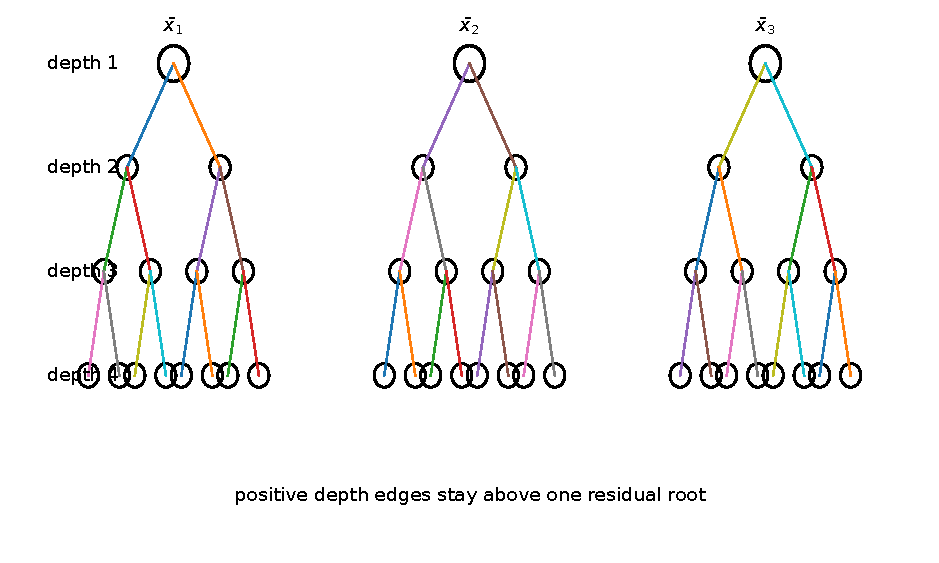
\includegraphics[width=.95\textwidth]{02_residual_forest.pdf}
\caption{Finite lift levels form a rooted forest. Every edge preserves the residual root.}
\label{fig:residual_forest}
\end{figure}

\section{Visibility filtrations and level counting}\label{sec:counting}

\subsection{Delayed separation of integral packets}

Let \(a_1,\ldots,a_s\in\OO\) be distinct integral coordinates. Their reductions may coincide at shallow precision even when the characteristic zero values are different.

\begin{definition}[Visibility partition]\label{def:visibility_partition}
For \(m\geq1\), define an equivalence relation on \(\{1,\ldots,s\}\) by
\[
i\sim_mj
\quad\Longleftrightarrow\quad
 a_i\equiv a_j\pmod{\varpi^m}.
\]
The resulting partition is the visible packet partition at depth \(m\).
\end{definition}

\begin{proposition}[Nested visibility]\label{prop:nested_visibility}
The depth \(m+1\) visibility partition refines the depth \(m\) partition.
\end{proposition}

\begin{proof}
Congruence modulo \(\varpi^{m+1}\) implies congruence modulo \(\varpi^m\).
\end{proof}

\begin{definition}[Separation depth]\label{def:separation_depth}
For \(i\neq j\), define
\[
w(i,j)
=
\min\{m\geq1:a_i\not\equiv a_j\pmod{\varpi^m}\}.
\]
Equivalently,
\[
w(i,j)=v_{\varpi}(a_i-a_j)+1.
\]
\end{definition}

\begin{proposition}[Ultrametric separation law]\label{prop:ultrametric_separation}
For distinct indices \(i,j,k\),
\[
\boxed{
w(i,k)\geq\min\{w(i,j),w(j,k)\}.}
\]
\end{proposition}

\begin{proof}
The nonarchimedean valuation satisfies
\[
v_{\varpi}(a_i-a_k)
\geq
\min\{v_{\varpi}(a_i-a_j),v_{\varpi}(a_j-a_k)\}.
\]
Add one to both sides.
\end{proof}

\begin{corollary}[Visibility cluster tree]\label{cor:visibility_tree}
The partitions in \cref{prop:nested_visibility} form a rooted tree. The leaves \(i\) and \(j\) first lie in different nodes at depth \(w(i,j)\).
\end{corollary}

\begin{proof}
Nested finite partitions define a rooted refinement tree. The definition of \(w(i,j)\) gives the first depth at which the two indices lie in different blocks.
\end{proof}

\begin{example}[Dyadic signs]\label{ex:dyadic_signs}
In \(\ZZ_2\), the points \(1\) and \(-1\) agree modulo \(2\) and differ modulo \(4\). Their separation depth is
\[
w(1,-1)=2.
\]
\end{example}

\begin{figure}[t]
\centering
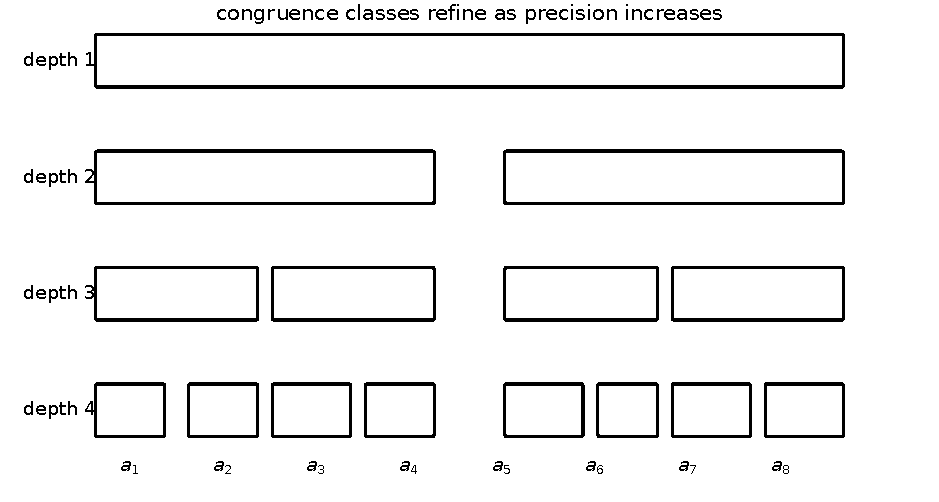
\includegraphics[width=.94\textwidth]{03_visibility_tree.pdf}
\caption{Integral packets may be indistinguishable at shallow depth and separate only after more precision is retained.}
\label{fig:visibility_tree}
\end{figure}

\subsection{Weighted formal charts}

\begin{definition}[Weighted formal chart]\label{def:weighted_chart}
Fix integers \(w_1,\ldots,w_d\geq1\). At depth \(m\), coordinate \(i\) ranges over
\[
\varpi^{w_i}\OO/\varpi^m.
\]
Write \(N_{\bm w}(m)\) for the number of coordinate tuples.
\end{definition}

\begin{proposition}[Weighted chart count]\label{prop:weighted_chart_count}
For every \(m\geq1\),
\[
\boxed{
N_{\bm w}(m)
=
q^{\sum_{i=1}^{d}\max(m-w_i,0)}.
}
\]
\end{proposition}

\begin{proof}
The quotient \(\varpi^{w_i}\OO/\varpi^m\) has one element when \(m\leq w_i\) and \(q^{m-w_i}\) elements when \(m>w_i\). Multiply the independent counts.
\end{proof}

\begin{definition}[Level counting series]\label{def:level_series}
For finite levels \(X_m\), define
\[
Z_X(T)
=
\sum_{m\geq1}\abs{X_m}T^m.
\]
When the limit exists, define the branching exponent
\[
\delta(X)
=
\lim_{m\to\infty}
\frac{\log_q\abs{X_m}}{m}.
\]
\end{definition}

\begin{theorem}[Smooth level series]\label{thm:smooth_level_series}
For a smooth formal chart of relative dimension \(d\),
\[
\boxed{
Z_d(T)
=
\frac{T}{1-q^dT},
\qquad
\delta=d.
}
\]
\end{theorem}

\begin{proof}
Insert \(\abs{X_m}=q^{d(m-1)}\) and sum the geometric series. The logarithmic growth is \(d(m-1)/m\), which tends to \(d\).
\end{proof}

\begin{theorem}[Weighted level series]\label{thm:weighted_level_series}
Assume
\[
1\leq w_1\leq\cdots\leq w_d.
\]
Put
\[
W=\sum_{i=1}^{d}w_i,
\qquad
w_{\max}=w_d.
\]
Then
\[
\boxed{
Z_{\bm w}(T)
=
\sum_{m=1}^{w_{\max}}
N_{\bm w}(m)T^m
+
q^{d(w_{\max}+1)-W}
\frac{T^{w_{\max}+1}}{1-q^dT}.
}
\]
Its branching exponent is \(d\).
\end{theorem}

\begin{proof}
For \(m\geq w_{\max}+1\), every coordinate is active and
\[
N_{\bm w}(m)=q^{dm-W}.
\]
The tail is geometric. The additive constant \(-W\) does not change the limiting slope.
\end{proof}

\subsection{Nilpotent and crossing charts}

\begin{theorem}[One power nilpotent chart]\label{thm:power_nilpotent}
In \(\OO/\varpi^m\), the equation
\[
x^e=0
\]
has exactly
\[
\boxed{
q^{m-\lceil m/e\rceil}
}
\]
solutions. Its level series is
\[
\boxed{
Z_e(T)
=
\frac{\sum_{r=1}^{e}q^{r-1}T^r}
{1-q^{e-1}T^e}.
}
\]
Its branching exponent is
\[
\boxed{
1-\frac1e.
}
\]
\end{theorem}

\begin{proof}
The congruence is equivalent to
\[
e v_{\varpi}(x)\geq m.
\]
Thus \(x\) lies in \(\varpi^{\lceil m/e\rceil}\OO/\varpi^m\), which has the stated size. Write \(m=ek+r\) with \(1\leq r\leq e\). Then
\[
m-\lceil m/e\rceil
=(e-1)k+r-1.
\]
Summation over \(k\) and \(r\) gives the rational expression. Division by \(m\) gives the branching exponent.
\end{proof}

\begin{theorem}[Diagonal nilpotent chart]\label{thm:diagonal_nilpotent}
Fix integers \(e_1,\ldots,e_d\geq1\). The system
\[
x_i^{e_i}=0
\qquad(1\leq i\leq d)
\]
in \((\OO/\varpi^m)^d\) has
\[
\boxed{
N_{\bm e}(m)
=
q^{\sum_{i=1}^{d}(m-\lceil m/e_i\rceil)}
}
\]
solutions. Let
\[
L=\operatorname{lcm}(e_1,\ldots,e_d)
\]
and
\[
D_L
=
\sum_{i=1}^{d}\left(L-\frac{L}{e_i}\right).
\]
Then
\[
\boxed{
Z_{\bm e}(T)
=
\frac{
\sum_{r=1}^{L}
q^{\sum_i(r-\lceil r/e_i\rceil)}T^r
}{1-q^{D_L}T^L}.
}
\]
The branching exponent is
\[
\boxed{
d-\sum_{i=1}^{d}\frac1{e_i}.
}
\]
\end{theorem}

\begin{proof}
The coordinates are independent, so \cref{thm:power_nilpotent} gives the product count. If \(m=Lk+r\) with \(1\leq r\leq L\), then
\[
\left\lceil\frac{m}{e_i}\right\rceil
=
\frac{L}{e_i}k
+
\left\lceil\frac{r}{e_i}\right\rceil.
\]
The exponent therefore increases by \(D_L\) when \(m\) increases by \(L\). This gives the rational series. The limiting slope is the displayed sum.
\end{proof}

\begin{theorem}[Normal crossing count]\label{thm:normal_crossing_count}
The number of pairs
\[
(x,y)\in(\OO/\varpi^m)^2
\]
satisfying
\[
xy=0
\]
is
\[
\boxed{
N_{\times}(m)
=
q^m+m(q-1)q^{m-1}.
}
\]
Its level series is
\[
\boxed{
Z_{\times}(T)
=
\frac{T(2q-1-q^2T)}{(1-qT)^2}.
}
\]
Its branching exponent is \(1\).
\end{theorem}

\begin{proof}
For \(0\leq a<m\), the number of \(x\) with valuation exactly \(a\) is
\[
(q-1)q^{m-a-1}.
\]
For such \(x\), the condition \(xy=0\) gives \(q^a\) choices for \(y\). Each valuation stratum therefore contributes \((q-1)q^{m-1}\). There are \(m\) such strata. The case \(x=0\) contributes \(q^m\). Summing the two geometric derivative series gives the rational formula. The factor \(m\) is subexponential, so the branching exponent is one.
\end{proof}

\begin{proposition}[Independent products]\label{prop:independent_products}
Suppose two finite level problems have counts \(A_m\) and \(B_m\), and their coordinate conditions are independent. The product problem has count
\[
N_m=A_mB_m.
\]
If the branching exponents of the two factors exist, the product exponent is their sum.
\end{proposition}

\begin{proof}
Independence gives the product count. Taking logarithms turns multiplication into addition, and division by \(m\) gives the exponent formula.
\end{proof}

\begin{figure}[t]
\centering
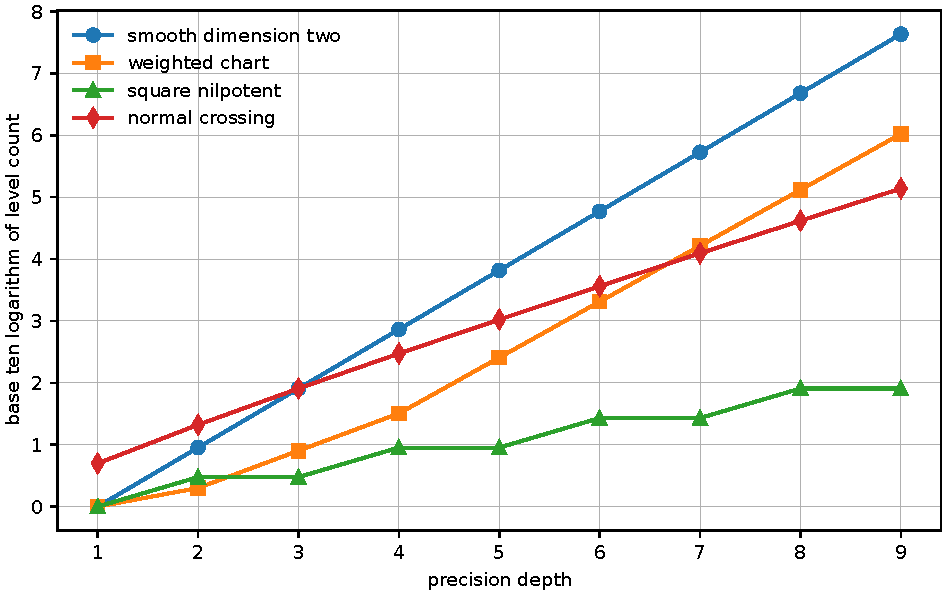
\includegraphics[width=.84\textwidth]{04_level_counts.pdf}
\caption{Smooth, weighted, nilpotent, and normal crossing charts have different finite depth counts. The logarithmic slopes record their branching exponents.}
\label{fig:level_counts}
\end{figure}

\section{Deformation complexes and packet obstructions}\label{sec:obstruction}

\subsection{Tangent and obstruction spaces}

Let
\[
\bar\rho:G\longrightarrow\GL_n(k)
\]
be a continuous residual representation. Write \(\ad\bar\rho\) for the adjoint module. The distinction between framed and unframed deformation problems is important. Framed first order deformations are described by cocycles, while unframed deformations under the usual Schur hypothesis are described by cohomology classes.

\begin{standardfact}[Galois tangent and obstruction spaces]\label{fact:galois_tangent_obstruction}
Under the standard finiteness and representability hypotheses, framed tangent directions are described by
\[
Z^1(G,\ad\bar\rho),
\]
unframed tangent directions are described by
\[
H^1(G,\ad\bar\rho),
\]
and a complete obstruction theory takes values in
\[
H^2(G,\ad\bar\rho).
\]
For a small extension with square zero kernel \(I\), the obstruction lies in
\[
H^2(G,\ad\bar\rho)\otimes_k I.
\]
When it vanishes, the lift set is a torsor under the corresponding first cohomology group. See \cite{Mazur1989,NeukirchSchmidtWingberg2008,Ramakrishna1993}.
\end{standardfact}

The statements below apply to any cochain complex, not only to Galois cochains.

\begin{definition}[Chain packet system]\label{def:chain_packets}
Let
\[
\cdots\longrightarrow C^{r-1}\xrightarrow{d^{r-1}}C^r\xrightarrow{d^r}C^{r+1}\longrightarrow\cdots
\]
be a cochain complex over a field. A finite chain packet system is a family of idempotents
\[
P_j^r:C^r\longrightarrow C^r
\]
such that
\[
\sum_jP_j^r=I,
\qquad
P_i^rP_j^r=\delta_{ij}P_j^r,
\qquad
 d^rP_j^r=P_j^{r+1}d^r.
\]
\end{definition}

\begin{theorem}[Cohomology packet decomposition]\label{thm:cohomology_packets}
Every packet in \cref{def:chain_packets} is a subcomplex and
\[
\boxed{
H^r(C^\bullet)
\cong
\bigoplus_jH^r(P_jC^\bullet).
}
\]
\end{theorem}

\begin{proof}
Commutation with the differential makes \(P_jC^\bullet\) a subcomplex. The direct sum decomposition of \(C^r\) restricts to
\[
\ker d^r
=
\bigoplus_j\ker(d^r|_{P_jC^r})
\]
and
\[
\im d^{r-1}
=
\bigoplus_j\im(d^{r-1}|_{P_jC^{r-1}}).
\]
Taking the quotient gives the result.
\end{proof}

\begin{corollary}[Tangent and obstruction packets]\label{cor:tangent_obstruction_packets}
Under the hypotheses of \cref{fact:galois_tangent_obstruction}, every chain packet system on the adjoint cochain complex gives
\[
H^1(G,\ad\bar\rho)
=
\bigoplus_jH^1_j
\]
and
\[
H^2(G,\ad\bar\rho)
=
\bigoplus_jH^2_j.
\]
\end{corollary}

\begin{proof}
Apply \cref{thm:cohomology_packets} in degrees one and two.
\end{proof}

\begin{figure}[t]
\centering
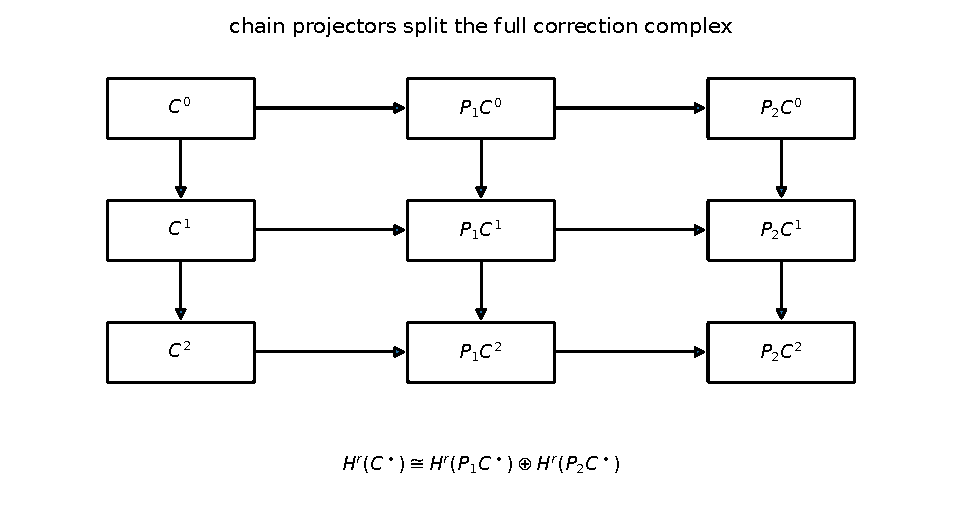
\includegraphics[width=.9\textwidth]{05_obstruction_packets.pdf}
\caption{Compatible chain projectors split the correction complex and therefore split both tangent and obstruction spaces.}
\label{fig:obstruction_packets}
\end{figure}

\subsection{Linear correction classes}

The universal obstruction attached to a linear correction map is a cokernel class.

\begin{definition}[Linear obstruction class]\label{def:linear_obstruction}
Let
\[
D:U\longrightarrow V
\]
be a linear map, and let \(r\in V\) be a residual defect. Define
\[
\Ob_D(r)
=
[r]
\in
\coker D.
\]
\end{definition}

\begin{theorem}[Linear lifting criterion]\label{thm:linear_lifting}
The correction equation
\[
Du=-r
\]
has a solution if and only if
\[
\boxed{
\Ob_D(r)=0.
}
\]
When one solution exists, the complete solution set is one coset of \(\ker D\).
\end{theorem}

\begin{proof}
The equation is solvable precisely when \(-r\in\im D\), which is equivalent to \([r]=0\) in the cokernel. If \(u_0\) is one solution, then every other solution is \(u_0+v\) with \(v\in\ker D\).
\end{proof}

\begin{corollary}[Finite field child count]\label{cor:finite_child_count}
Let \(U\) and \(V\) be finite dimensional vector spaces over \(\FF_q\). If the obstruction vanishes, the correction equation has exactly
\[
\boxed{
q^{\dim\ker D}
}
\]
solutions.
\end{corollary}

\begin{proof}
The solution set is a coset of \(\ker D\), and a vector space of dimension \(d\) over \(\FF_q\) has \(q^d\) elements.
\end{proof}

\begin{theorem}[Packetwise lifting criterion]\label{thm:packetwise_lifting}
Suppose
\[
U=\bigoplus_jU_j,
\qquad
V=\bigoplus_jV_j,
\]
and
\[
D(U_j)\subseteq V_j.
\]
Write \(r=\sum_jr_j\). Then
\[
\boxed{
\Ob_D(r)=0
\quad\Longleftrightarrow\quad
[r_j]=0\text{ in }\coker(D|_{U_j})
\text{ for every }j.
}
\]
\end{theorem}

\begin{proof}
The map \(D\) is the direct sum of its restrictions. Therefore
\[
\coker D
\cong
\bigoplus_j\coker(D|_{U_j}),
\]
and the class of \(r\) is the tuple of the classes of the \(r_j\).
\end{proof}

\begin{corollary}[Packet child count]\label{cor:packet_child_count}
Under the finite field hypotheses of \cref{cor:finite_child_count,thm:packetwise_lifting}, a lift exists if and only if every packet obstruction vanishes. When it exists, the number of correction classes is
\[
\boxed{
q^{\sum_j\dim\ker(D|_{U_j})}.
}
\]
\end{corollary}

\begin{proof}
Use \cref{thm:packetwise_lifting} and multiply the packetwise kernel counts.
\end{proof}

\subsection{Small extensions and obstruction torsors}

\begin{definition}[Complete obstruction theory]\label{def:complete_obstruction_theory}
Let \(\calF\) be a deformation functor. A complete obstruction theory assigns to every small extension
\[
0\longrightarrow I\longrightarrow A'\longrightarrow A\longrightarrow0
\]
and every \(x\in\calF(A)\) a class
\[
\omega(x,A'/A)\in O_x\otimes_kI
\]
such that the class vanishes exactly when \(x\) lifts to \(A'\). When the class vanishes, the lift set is a torsor under a declared tangent space \(T_x\otimes_kI\).
\end{definition}

\begin{proposition}[Packet obstruction torsor]\label{prop:packet_obstruction_torsor}
Suppose a complete obstruction theory has decompositions
\[
T_x=\bigoplus_jT_{x,j},
\qquad
O_x=\bigoplus_jO_{x,j},
\]
and the obstruction class decomposes accordingly. Then a lift exists if and only if every packet component of the obstruction vanishes. If \(k\) is finite and the lift set is nonempty, its cardinality is
\[
\boxed{
q^{(\dim_kI)\sum_j\dim_kT_{x,j}}.
}
\]
\end{proposition}

\begin{proof}
A vector in a direct sum is zero exactly when every component is zero. The torsor has the same cardinality as
\[
T_x\otimes_kI,
\]
whose dimension is \((\dim_kI)\sum_j\dim_kT_{x,j}\).
\end{proof}

\begin{corollary}[Unobstructed packet problem]\label{cor:unobstructed_packet}
Suppose \(O_{x,j}=0\) for every \(j\). Then every small extension in the declared theory admits a lift.
\end{corollary}

\begin{proof}
Every obstruction class lies in the zero vector space, so it vanishes. Apply \cref{def:complete_obstruction_theory}.
\end{proof}

\begin{remark}\label{rem:h2_boundary}
The vanishing of a group called \(H^2\) implies formal smoothness only when that group is part of a complete obstruction theory for the declared functor. The cohomology label alone is not enough.
\end{remark}

\section{Residual transport and directed generation}\label{sec:transport}

Vertical lifting remains above one residual root. A horizontal operation must therefore be recorded separately.

\begin{definition}[Admissible residual transport]\label{def:residual_transport}
Let \(\bar x\) and \(\bar y\) be residual roots with lift systems \((X_m)\) and \((Y_m)\). An admissible transport from \(\bar x\) to \(\bar y\) is a family of maps
\[
\tau_m:X_m\longrightarrow Y_m
\]
that commutes with every reduction map and preserves the declared determinant, local condition, and arithmetic spine data.
\end{definition}

\begin{proposition}[Transport of branches]\label{prop:transport_branches}
An admissible residual transport induces a map
\[
\boxed{
\varprojlim_mX_m
\longrightarrow
\varprojlim_mY_m.
}
\]
\end{proposition}

\begin{proof}
If \((x_m)\) is compatible, then commutation with reduction gives
\[
r^Y_{m+1,m}(\tau_{m+1}(x_{m+1}))
=
\tau_m(r^X_{m+1,m}(x_{m+1}))
=
\tau_m(x_m).
\]
Thus \((\tau_m(x_m))\) is a compatible branch.
\end{proof}

\begin{definition}[Residual transport graph]\label{def:transport_graph}
For a finite set of residual roots, form a directed graph \(\Gamma\) with one vertex for each root and one edge for each declared admissible transport. A set of starting roots generates the vertices reachable by directed paths.
\end{definition}

\begin{definition}[Directed residual rank]\label{def:directed_rank}
The directed residual rank of \(\Gamma\) is the least cardinality of a vertex set whose directed closure is all of \(\Gamma\).
\end{definition}

\begin{theorem}[Source component theorem]\label{thm:source_scc}
Let \(\Gamma\) be a finite directed graph. Its directed residual rank is the number of source strongly connected components in its condensation graph.
\end{theorem}

\begin{proof}
A source component has no incoming edge from another component. Any generating set must therefore meet every source component. This gives the lower bound. Choose one vertex in each source component. Every component of a finite acyclic condensation graph is reachable from a source component. Strong connectivity allows the chosen vertex to reach every vertex in its own component. The selected vertices therefore generate all of \(\Gamma\).
\end{proof}

\begin{corollary}[One residual generator]\label{cor:one_residual_generator}
A finite residual transport graph has directed residual rank one if and only if its condensation graph has exactly one source component.
\end{corollary}

\begin{proof}
Apply \cref{thm:source_scc}.
\end{proof}

\begin{proposition}[Transport preserves obstruction vanishing]\label{prop:transport_obstruction}
Suppose an admissible transport is induced by a commuting square of correction maps
\[
\begin{CD}
U_X @>{D_X}>> V_X\\
@V{f}VV @VV{g}V\\
U_Y @>{D_Y}>> V_Y.
\end{CD}
\]
Then \(g\) induces a map
\[
\coker D_X\longrightarrow\coker D_Y.
\]
If a defect is correctable before transport, its transported defect is correctable after transport.
\end{proposition}

\begin{proof}
The equality \(gD_X=D_Yf\) shows that \(g(\im D_X)\subseteq\im D_Y\), so \(g\) descends to cokernels. A zero class maps to a zero class.
\end{proof}

\begin{remark}\label{rem:graph_boundary}
The source component theorem counts generators among roots that already exist. It does not prove that the required residual roots exist, that an admissible transport exists between them, or that transport preserves global occupancy.
\end{remark}

\begin{figure}[t]
\centering
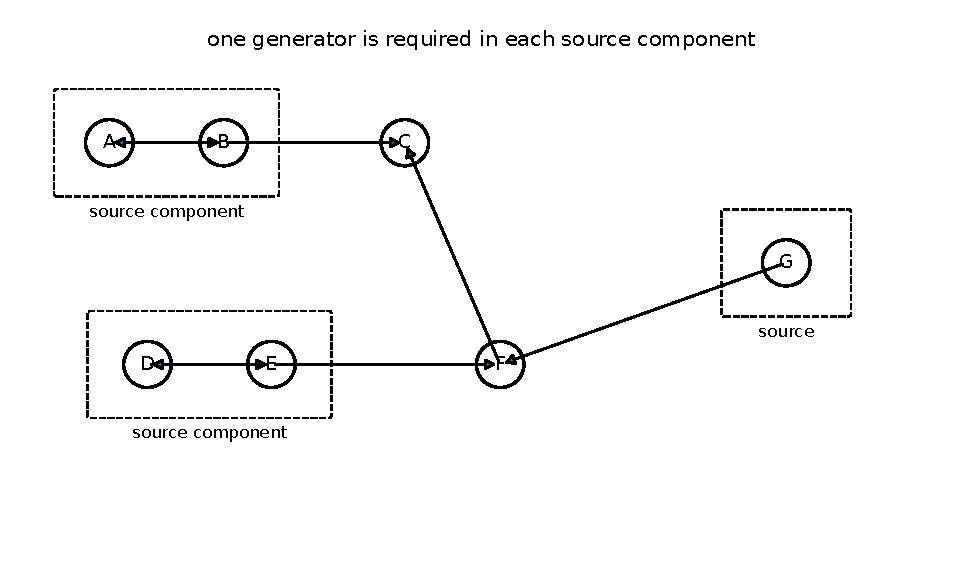
\includegraphics[width=.9\textwidth]{06_transport_graph.pdf}
\caption{The finite transport graph has three source components. One starting root is required in each.}
\label{fig:transport_graph}
\end{figure}

\section{Companion forests and common arithmetic spines}\label{sec:companions}

\subsection{Strict compatibility data}

Let \(E\) be a number field. Let \(\Lambda\) be a set of finite places of \(E\). Fix a number field \(F\), a finite set \(S\) of places of \(F\), and an integer \(n\). The profinite and continuous representation conventions are standard \cite{RibesZalesskii2010}.

\begin{definition}[Common arithmetic spine]\label{def:common_spine}
A common arithmetic spine \(\mathfrakC\) consists of the following declared data.
\begin{enumerate}
\item For every finite place \(v\notin S\), a monic polynomial
\[
P_v(X)\in E[X]
\]
of degree \(n\).
\item A determinant character or determinant polynomial compatible with the \(P_v\).
\item Selected local labels at the places in \(S\), such as inertial type, monodromy type, or another fixed local deformation condition.
\item Any weight or Hodge data that are required in the chosen arithmetic class.
\end{enumerate}
\end{definition}

\begin{definition}[Strictly compatible realization]\label{def:strict_compatible_realization}
A family
\[
\{\rho_\lambda\}_{\lambda\in\Lambda}
\]
of continuous semisimple representations
\[
\rho_\lambda:G_{F,S}\longrightarrow\GL_n(E_\lambda)
\]
realizes \(\mathfrakC\) if, for every \(v\notin S\) whose residue characteristic differs from that of \(\lambda\),
\[
\det\bigl(X-\rho_\lambda(\Frob_v)\bigr)
=
P_v(X)
\]
under the embedding \(E\hookrightarrow E_\lambda\), and if the selected local data are satisfied.
\end{definition}

This is the standard shape of strict compatibility used in the literature on compatible systems \cite{Serre1998,LarsenPink1992,BellaicheChenevier2009}.

\subsection{Finite companion levels}

For each \(\lambda\in\Lambda\), let \(\OO_\lambda\) be the valuation ring of \(E_\lambda\), with maximal ideal generated by \(\varpi_\lambda\).

\begin{definition}[Companion level]\label{def:companion_level}
Let
\[
X_{\lambda,m}(\mathfrakC)
\]
be the finite set of admissible objects over
\[
\OO_\lambda/\varpi_\lambda^m
\]
that realize the reduction of the declared spine and local conditions at precision \(m\). Reduction gives a companion forest
\[
\cdots\longrightarrow X_{\lambda,3}(\mathfrakC)
\longrightarrow X_{\lambda,2}(\mathfrakC)
\longrightarrow X_{\lambda,1}(\mathfrakC).
\]
\end{definition}

\begin{theorem}[One place companion completion]\label{thm:one_place_completion}
Fix \(\lambda\). Suppose the finite inverse system \(X_{\lambda,m}(\mathfrakC)\) satisfies the Mittag Leffler condition and has nonempty stable core at every depth. Then it has a complete branch.
\end{theorem}

\begin{proof}
Apply \cref{thm:finite_ml_branch}.
\end{proof}

\begin{corollary}[Empty companion obstruction]\label{cor:empty_companion}
If
\[
X_{\lambda,m}(\mathfrakC)=\varnothing
\]
for one coefficient place \(\lambda\) and one depth \(m\), then no strictly compatible realization of \(\mathfrakC\) exists at all places in \(\Lambda\).
\end{corollary}

\begin{proof}
Any \(\lambda\) adic realization would reduce to an element of every finite level. An empty level rules this out.
\end{proof}

\begin{theorem}[Simultaneous companion completion]\label{thm:simultaneous_completion}
Suppose that, for every \(\lambda\in\Lambda\), the companion forest has a nonempty compact inverse limit that is identified with complete local realizations
\[
X_\lambda(\mathfrakC)
=
\varprojlim_mX_{\lambda,m}(\mathfrakC).
\]
Then
\[
\boxed{
\prod_{\lambda\in\Lambda}
X_\lambda(\mathfrakC)
\neq
\varnothing.
}
\]
Every point of this product is a simultaneous family realizing the common spine.
\end{theorem}

\begin{proof}
Each factor is nonempty and compact. Tychonoff's theorem gives a nonempty compact product \cite{Kelley1955}. Every coordinate realizes the same declared spine by the definition of the factor.
\end{proof}

\begin{corollary}[Finite place completion]\label{cor:finite_place_completion}
If \(\Lambda\) is finite and every local companion forest satisfies the hypotheses of \cref{thm:one_place_completion}, then a simultaneous family exists.
\end{corollary}

\begin{proof}
Each factor is nonempty. A finite product of nonempty sets is nonempty.
\end{proof}

\begin{proposition}[Closed local conditions survive completion]\label{prop:closed_local_conditions}
Suppose each finite level is cut out inside an ambient compact inverse system by conditions whose inverse limit is closed. Every branch selected from the companion forest satisfies the limiting local condition.
\end{proposition}

\begin{proof}
A branch belongs to every finite condition set. Its image in the ambient inverse limit lies in their inverse limit, which is the declared closed limiting condition.
\end{proof}

\begin{theorem}[Exact recovery of the spine]\label{thm:spine_recovery}
Let \((\rho_{\lambda,m})_m\) be a complete branch. Suppose that for every unramified place \(v\notin S\),
\[
\det\bigl(X-\rho_{\lambda,m}(\Frob_v)\bigr)
\equiv
P_v(X)
\pmod{\varpi_\lambda^m}
\]
for every \(m\). Then the limiting representation satisfies
\[
\boxed{
\det\bigl(X-\rho_\lambda(\Frob_v)\bigr)
=
P_v(X)
}
\]
in \(E_\lambda[X]\).
\end{theorem}

\begin{proof}
The coefficients of the two monic polynomials agree modulo every power of \(\varpi_\lambda\). The coefficient ring is separated, so they are equal.
\end{proof}

\begin{example}[The equation \(x^2+1=0\)]\label{ex:x2plus1}
The finite companion forests for the scalar equation \(x^2+1=0\) illustrate the residual obstruction. At the primes \(5\) and \(13\), two simple residual roots lift through every tested depth. At the prime \(2\), the root modulo \(2\) has no child modulo \(4\). At the primes \(3\) and \(7\), there is no residual root. A complete branch at one prime does not create a branch at another prime.
\end{example}

\begin{figure}[t]
\centering
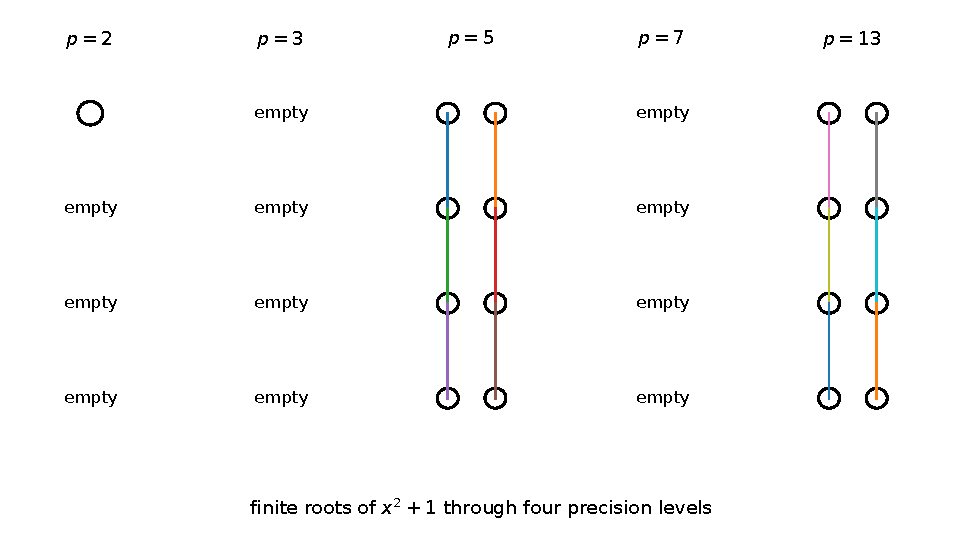
\includegraphics[width=.94\textwidth]{07_companion_forests.pdf}
\caption{Finite companion forests for \(x^2+1=0\). The obstruction can occur at residual depth or at the next precision level.}
\label{fig:companion_forests}
\end{figure}

\begin{figure}[t]
\centering
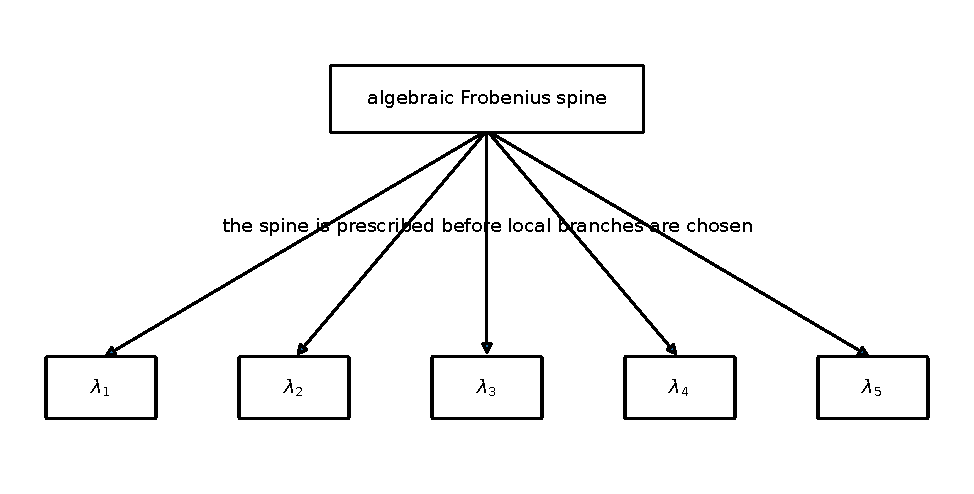
\includegraphics[width=.92\textwidth]{08_common_spine.pdf}
\caption{A common spine is fixed before the local branches are chosen. Nonemptiness of the local fibers is a separate theorem or hypothesis.}
\label{fig:common_spine}
\end{figure}

\section{Finite Frobenius separation and compatible carriers}\label{sec:frobenius}

\subsection{Separation by finitely many places}

The following argument combines character independence with Chebotarev density. We use the standard forms of these results from \cite{CurtisReiner1962,Serre1977,Neukirch1999}.

\begin{standardfact}[Chebotarev and Brauer Nesbitt]\label{fact:chebotarev_bn}
Frobenius conjugacy classes at unramified places are dense in the relevant profinite Galois group. Finite dimensional semisimple representations in characteristic zero are determined by their characters. Pairwise nonisomorphic absolutely irreducible representations have linearly independent characters.
\end{standardfact}

\begin{theorem}[Finite Frobenius trace separation]\label{thm:frobenius_separation}
Let
\[
\mathcal W_1,\ldots,\mathcal W_r
\]
be strictly compatible systems over \(E\). Suppose that, at one coefficient place \(\lambda_0\), the members
\[
W_{1,\lambda_0},\ldots,W_{r,\lambda_0}
\]
are pairwise nonisomorphic and absolutely irreducible. Then there are finitely many unramified places
\[
v_1,\ldots,v_s
\]
such that the matrix
\[
C
=
\left(
\Tr W_{i,\lambda}(\Frob_{v_j})
\right)_{
1\leq j\leq s,
1\leq i\leq r}
\]
has column rank \(r\). Its entries lie in \(E\) and are independent of \(\lambda\).
\end{theorem}

\begin{proof}
Fix \(\lambda_0\). The characters of the \(W_{i,\lambda_0}\) are linearly independent by \cref{fact:chebotarev_bn}. Their restrictions to the dense set of unramified Frobenius classes remain linearly independent. Otherwise a nonzero linear combination would vanish on a dense set and therefore everywhere by continuity. A finite family of linearly independent functions has a finite set of evaluation points on which the evaluation matrix has full column rank. Choose these points among Frobenius classes. Strict compatibility places every trace in \(E\) and makes it independent of \(\lambda\).
\end{proof}

\begin{corollary}[Finite trace determination]\label{cor:finite_trace_determination}
Under the hypotheses of \cref{thm:frobenius_separation}, a multiplicity vector
\[
\bm m=(m_1,\ldots,m_r)^T
\]
is uniquely determined by the finite trace vector
\[
\bm t=C\bm m.
\]
\end{corollary}

\begin{proof}
The matrix \(C\) has trivial kernel.
\end{proof}

\begin{theorem}[Compatible carrier summand]\label{thm:compatible_carrier}
Suppose a semisimple strictly compatible carrier has a decomposition
\[
\mathcal W
\cong
\bigoplus_{i=1}^{r}
\mathcal W_i^{\oplus c_i},
\]
where the \(\mathcal W_i\) satisfy the hypotheses of \cref{thm:frobenius_separation}. Suppose also that the declared local conditions are stable under the direct sums and summands appearing below. Let
\[
0\leq m_i\leq c_i
\]
be integers. Then
\[
\boxed{
\mathcal V
=
\bigoplus_{i=1}^{r}
\mathcal W_i^{\oplus m_i}
}
\]
is a strictly compatible summand of \(\mathcal W\). Its multiplicity vector is uniquely recoverable from the finite trace separator.
\end{theorem}

\begin{proof}
At every coefficient place, use the same multiplicities \(m_i\). Direct sums preserve the characteristic polynomials and local data required for strict compatibility. The inequalities \(m_i\leq c_i\) make the result a summand. Uniqueness follows from \cref{cor:finite_trace_determination}.
\end{proof}

\begin{corollary}[One member propagation inside a known carrier]\label{cor:one_member_propagation}
Suppose a semisimple summand at one coefficient place has decomposition
\[
V_{\lambda_0}
\cong
\bigoplus_iW_{i,\lambda_0}^{\oplus m_i}
\]
inside the declared compatible carrier. Then the same multiplicities define a strictly compatible summand at every coefficient place.
\end{corollary}

\begin{proof}
Apply \cref{thm:compatible_carrier}.
\end{proof}

\begin{proposition}[Field extension invariance]\label{prop:field_extension_separator}
The rank of a finite Frobenius separator matrix is unchanged after extending the coefficient field.
\end{proposition}

\begin{proof}
A maximal minor is zero before extension exactly when its image is zero after an injective field extension. The largest size of a nonzero minor is therefore unchanged.
\end{proof}

\begin{remark}\label{rem:carrier_boundary}
The carrier theorem is conditional on a known compatible decomposition. It does not prove that an arbitrary geometric representation embeds into such a carrier.
\end{remark}

\begin{figure}[t]
\centering
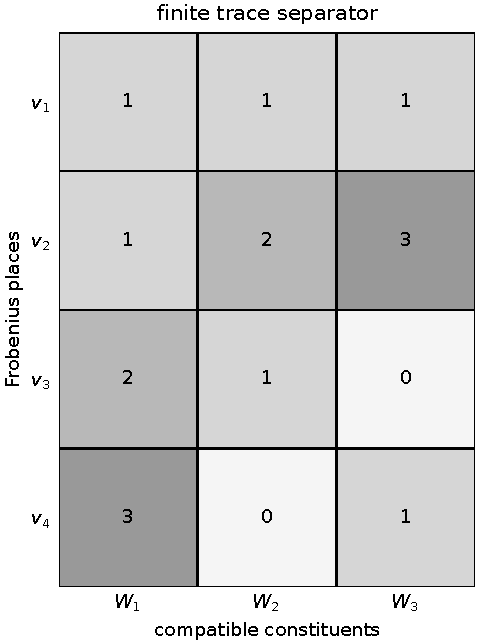
\includegraphics[width=.72\textwidth]{09_frobenius_separator.pdf}
\caption{A finite collection of Frobenius traces separates the compatible constituents and recovers their multiplicities.}
\label{fig:frobenius_separator}
\end{figure}

\section{Support occupancy over commutative rings}\label{sec:support}

Finite spectral projectors are effective when the carrier is semisimple. Deformation rings, patched modules, and Hecke algebras are usually not semisimple. Module support gives a definition that survives nilpotents, singularities, and specialization.

\subsection{Support and Fitting ideals}

Let \(R\) be a commutative Noetherian ring and let \(M\) be a finite \(R\) module.

\begin{definition}[Support occupancy]\label{def:support_occupancy}
The occupied locus of \(M\) is its support
\[
\Supp_R(M)
=
\{\mathfrak p\in\Spec R:M_{\mathfrak p}\neq0\}.
\]
A component, point, or packet of \(\Spec R\) is occupied when it meets this support.
\end{definition}

\begin{standardfact}[Support and annihilator]\label{fact:support_ann}
For a finite module over a Noetherian ring,
\[
\boxed{
\Supp_R(M)
=
V(\Ann_R(M)).
}
\]
The support is closed and stable under specialization. See \cite{AtiyahMacdonald1969,Eisenbud1995,Matsumura1989}.
\end{standardfact}

Choose a finite presentation
\[
R^a\xrightarrow{\Phi}R^b\longrightarrow M\longrightarrow0.
\]
The zeroth Fitting ideal is generated by the \(b\) by \(b\) minors of \(\Phi\), with the usual conventions when \(a<b\).

\begin{theorem}[Fitting support theorem]\label{thm:fitting_support}
For every finite \(R\) module,
\[
\boxed{
\Supp_R(M)
=
V\bigl(\Fitt_0^R(M)\bigr).
}
\]
\end{theorem}

\begin{proof}
Localize at \(\mathfrak p\). The localized module is zero exactly when the localized presentation map is surjective. A map into \(R_{\mathfrak p}^b\) is surjective exactly when one maximal minor is a unit. This is equivalent to
\[
\Fitt_0^R(M)R_{\mathfrak p}=R_{\mathfrak p}.
\]
Thus \(M_{\mathfrak p}\neq0\) exactly when \(\Fitt_0^R(M)\subseteq\mathfrak p\).
\end{proof}

\begin{corollary}[Occupancy from a presentation]\label{cor:occupancy_minors}
A prime \(\mathfrak p\) is occupied exactly when every maximal presentation minor lies in \(\mathfrak p\).
\end{corollary}

\begin{proof}
This is the pointwise form of \cref{thm:fitting_support}.
\end{proof}

\begin{proposition}[Local fiber criterion]\label{prop:local_fiber_criterion}
For every prime \(\mathfrak p\),
\[
\boxed{
\mathfrak p\in\Supp_R(M)
\quad\Longleftrightarrow\quad
M\otimes_R\kappa(\mathfrak p)\neq0.
}
\]
\end{proposition}

\begin{proof}
The fiber is
\[
M_{\mathfrak p}/\mathfrak pM_{\mathfrak p}.
\]
If \(M_{\mathfrak p}=0\), the fiber is zero. Conversely, if the fiber is zero, Nakayama's lemma gives \(M_{\mathfrak p}=0\).
\end{proof}

\begin{theorem}[Generator strata from higher Fitting ideals]\label{thm:fitting_generator_strata}
Let
\[
\mu_{\mathfrak p}(M)
=
\dim_{\kappa(\mathfrak p)}
M\otimes_R\kappa(\mathfrak p).
\]
For every integer \(r\geq1\),
\[
\boxed{
\{\mathfrak p:\mu_{\mathfrak p}(M)\geq r\}
=
V\bigl(\Fitt_{r-1}^R(M)\bigr).
}
\]
\end{theorem}

\begin{proof}
After localization at \(\mathfrak p\), the number \(\mu_{\mathfrak p}(M)\) is the minimum number of generators of \(M_{\mathfrak p}\). A finite presentation matrix has rank at most \(b-r\) over the residue field exactly when all minors of size \(b-r+1\) vanish. By the definition of Fitting ideals, this is equivalent to \(\Fitt_{r-1}(M)\subseteq\mathfrak p\).
\end{proof}

\begin{corollary}[Closed multiplicity loci]\label{cor:closed_multiplicity_loci}
For a finite module, the locus where the fiber requires at least \(r\) generators is closed.
\end{corollary}

\begin{proof}
It is the vanishing locus in \cref{thm:fitting_generator_strata}.
\end{proof}

\begin{figure}[t]
\centering
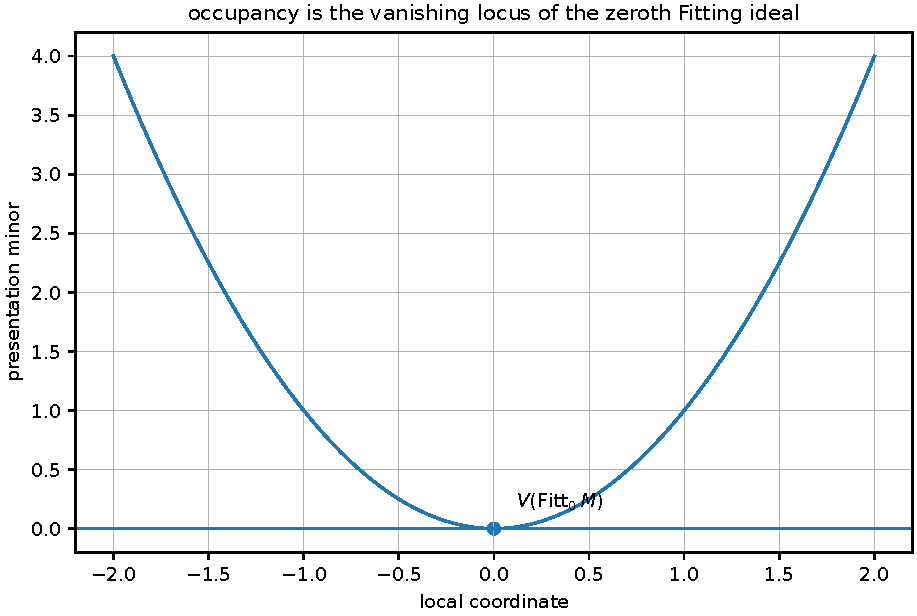
\includegraphics[width=.74\textwidth]{11_fitting_locus.pdf}
\caption{The occupied locus is the vanishing set of the zeroth Fitting ideal. Higher Fitting ideals record fiber multiplicity strata.}
\label{fig:fitting_locus}
\end{figure}

\subsection{Idempotent components}

\begin{definition}[Ring packet decomposition]\label{def:ring_packets}
Suppose
\[
R
\cong
R_1\times\cdots\times R_s.
\]
Let \(e_i\in R\) be the central idempotent selecting the \(i\)th factor. For an \(R\) module \(M\), the component \(i\) is occupied when
\[
e_iM\neq0.
\]
\end{definition}

\begin{theorem}[Exact idempotent decomposition]\label{thm:idempotent_decomposition}
Every \(R\) module has a canonical decomposition
\[
\boxed{
M
=
\bigoplus_{i=1}^{s}e_iM.
}
\]
Its support is the disjoint union of the supports of the occupied components inside
\[
\Spec R
=
\coprod_{i=1}^{s}\Spec R_i.
\]
\end{theorem}

\begin{proof}
The idempotents are orthogonal and sum to one. Therefore every \(m\in M\) has the unique decomposition
\[
m=\sum_ie_im.
\]
Localization on the \(i\)th component kills every \(e_jM\) with \(j\neq i\), so the support decomposes in the same way.
\end{proof}

\begin{corollary}[Faithfulness occupies every factor]\label{cor:faithful_components}
If \(M\) is faithful and every factor ring \(R_i\) is nonzero, then
\[
e_iM\neq0
\]
for every \(i\).
\end{corollary}

\begin{proof}
If \(e_iM=0\), then the nonzero idempotent \(e_i\) belongs to \(\Ann_R(M)\), contradicting faithfulness.
\end{proof}

\begin{proposition}[Full support criterion]\label{prop:full_support}
For a finite \(R\) module,
\[
\Supp_R(M)=\Spec R
\]
if and only if
\[
\sqrt{\Ann_R(M)}
=
\sqrt{(0)}.
\]
Faithfulness is sufficient but not necessary.
\end{proposition}

\begin{proof}
By \cref{fact:support_ann}, full support is equivalent to
\[
V(\Ann_R(M))=V(0).
\]
Two ideals have the same vanishing set exactly when they have the same radical.
\end{proof}

\begin{example}[Full support without faithfulness]\label{ex:full_support_not_faithful}
Let
\[
R=k[\epsilon]/(\epsilon^2)
\]
and
\[
M=R/(\epsilon).
\]
Then \(\Ann_R(M)=(\epsilon)\neq0\), so \(M\) is not faithful. Both \((\epsilon)\) and \((0)\) have the same radical, and \(\Spec R\) has one point. Thus \(M\) has full support.
\end{example}

\begin{figure}[t]
\centering
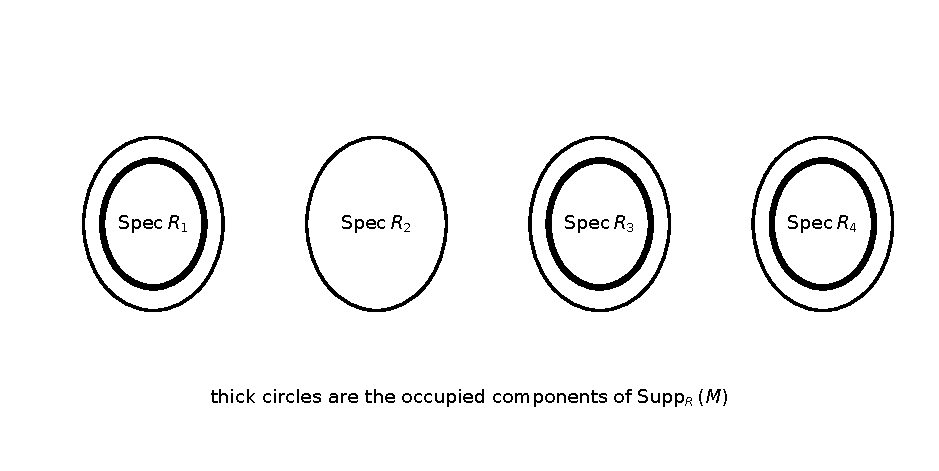
\includegraphics[width=.9\textwidth]{10_support_components.pdf}
\caption{A product ring separates its components by central idempotents. Support records which components are actually occupied.}
\label{fig:support_components}
\end{figure}

\subsection{Base change and specialization}

\begin{proposition}[Support under arbitrary base change]\label{prop:support_arbitrary_base_change}
Let \(R\to S\) be a ring map. Then
\[
\boxed{
\Supp_S(M\otimes_RS)
\subseteq
\{\mathfrak q\in\Spec S:\mathfrak q\cap R\in\Supp_R(M)\}.
}
\]
\end{proposition}

\begin{proof}
Let \(\mathfrak q\in\Spec S\) and put \(\mathfrak p=\mathfrak q\cap R\). If \(M_{\mathfrak p}=0\), then
\[
(M\otimes_RS)_{\mathfrak q}
\cong
M_{\mathfrak p}\otimes_{R_{\mathfrak p}}S_{\mathfrak q}
=0.
\]
\end{proof}

\begin{theorem}[Flat base change of support]\label{thm:flat_base_change_support}
If \(R\to S\) is flat, then
\[
\boxed{
\Supp_S(M\otimes_RS)
=
\{\mathfrak q\in\Spec S:\mathfrak q\cap R\in\Supp_R(M)\}.
}
\]
\end{theorem}

\begin{proof}
Only the reverse inclusion remains. Let \(\mathfrak p\in\Supp_R(M)\) and let \(\mathfrak q\) lie above \(\mathfrak p\). The local map
\[
R_{\mathfrak p}\longrightarrow S_{\mathfrak q}
\]
is flat and local, hence faithfully flat. Since \(M_{\mathfrak p}\neq0\), its tensor product with \(S_{\mathfrak q}\) is nonzero.
\end{proof}

\begin{corollary}[Faithfully flat detection]\label{cor:faithfully_flat_detection}
If \(R\to S\) is faithfully flat, then
\[
M=0
\quad\Longleftrightarrow\quad
M\otimes_RS=0.
\]
\end{corollary}

\begin{proof}
The map \(\Spec S\to\Spec R\) is surjective. Apply \cref{thm:flat_base_change_support}.
\end{proof}

\begin{proposition}[Specialization closure]\label{prop:specialization_closure}
Suppose \(\mathfrak p\subseteq\mathfrak q\) and \(\mathfrak p\in\Supp_R(M)\). Then
\[
\mathfrak q\in\Supp_R(M).
\]
\end{proposition}

\begin{proof}
The support is \(V(\Ann_R(M))\). Every prime containing \(\mathfrak p\) also contains \(\Ann_R(M)\).
\end{proof}

\section{Finite and Artinian occupancy}\label{sec:finiteoccupancy}

\subsection{Artinian packet algebras}

Let \(E\) be a field of characteristic zero and let \(A\) be a finite dimensional commutative \(E\) algebra. Such an algebra has a canonical decomposition into local Artinian factors
\[
A
\cong
A_1\times\cdots\times A_s.
\]
Let \(e_i\) denote the associated central idempotents.

\begin{theorem}[Artinian packet occupancy]\label{thm:artinian_occupancy}
For every finite dimensional \(A\) module \(V\),
\[
\boxed{
V
=
\bigoplus_{i=1}^{s}e_iV.
}
\]
The \(i\)th Artinian packet is occupied exactly when \(e_iV\neq0\). As an \(E\) linear operator,
\[
\boxed{
\Tr_E(e_i|_V)
=
\dim_E(e_iV)\,1_E,
\qquad
\rank_E(e_i|_V)
=
\dim_E(e_iV).
}
\]
\end{theorem}

\begin{proof}
The module decomposition follows from \cref{thm:idempotent_decomposition}. An idempotent linear operator is diagonalizable with eigenvalues zero and one. Its one eigenspace is \(e_iV\). The trace is the image of its dimension in \(E\), and the rank is its dimension.
\end{proof}

\begin{corollary}[Nonsemisimple packet trace]\label{cor:nonsemisimple_packet_trace}
Trace detects a central Artinian packet over any field of characteristic zero. Neither the algebra nor its action must be semisimple. An exact central idempotent is enough.
\end{corollary}

\begin{proof}
The proof of \cref{thm:artinian_occupancy} uses idempotency and finite dimension, not semisimplicity.
\end{proof}

\subsection{Commuting semisimple operators}

Let \(T_1,\ldots,T_N\) be commuting split semisimple operators on a finite dimensional vector space \(V\) over \(E\). Fix selected eigenvalues \(a_i\in E\).

\begin{definition}[Joint spectral packet]\label{def:joint_spectral_packet}
For each \(i\), define
\[
e_i
=
\prod_{\mu\in\Spec(T_i)\setminus\{a_i\}}
\frac{T_i-\mu I}{a_i-\mu}
\]
when \(a_i\in\Spec(T_i)\), and put \(e_i=0\) otherwise. Define
\[
e_{\bm a}
=
\prod_{i=1}^{N}e_i.
\]
\end{definition}

\begin{theorem}[Exact joint occupancy projector]\label{thm:joint_occupancy}
The operator \(e_{\bm a}\) is the projector onto
\[
V_{\bm a}
=
\{v\in V:T_iv=a_iv\text{ for every }i\}.
\]
In particular,
\[
\boxed{
\Tr_E(e_{\bm a})
=
\dim_E(V_{\bm a})\,1_E,
\qquad
\rank_E(e_{\bm a})
=
\dim_E(V_{\bm a}).
}
\]
The joint packet is occupied exactly when its rank is positive, equivalently when its trace is nonzero.
\end{theorem}

\begin{proof}
The Lagrange polynomial defining \(e_i\) equals one on the \(a_i\) eigenspace and zero on every other eigenspace. The operators commute, so the projectors commute. Their product projects onto the intersection of the selected eigenspaces. The trace is the image of the packet dimension in \(E\), and the rank is the packet dimension.
\end{proof}

\begin{corollary}[Monotone finite ranks]\label{cor:monotone_finite_ranks}
Let \((e_i)_{i\geq1}\) be a sequence of pairwise commuting idempotents on a fixed finite dimensional vector space, and set
\[
E_m=e_1e_2\cdots e_m.
\]
Then
\[
\rank E_{m+1}\leq\rank E_m.
\]
If \(\rank E_m>0\) for every \(m\), then
\[
\bigcap_{m\geq1}\im E_m
\neq0.
\]
\end{corollary}

\begin{proof}
The range of \(E_{m+1}\) is contained in the range of \(E_m\). The nonnegative integer ranks form a descending sequence and therefore stabilize. Once the ranks stabilize, the nested ranges are equal. Their common stabilized value is the infinite intersection, and it is nonzero because every rank is positive.
\end{proof}

\begin{proposition}[Support interpretation of a joint packet]\label{prop:support_joint_packet}
Let
\[
B=E[T_1,\ldots,T_N]
\subseteq
\End_E(V).
\]
Since the \(T_i\) commute and are split semisimple, \(B\) is a finite dimensional commutative semisimple algebra. Its maximal ideals correspond to joint eigencharacters. If the selected tuple \(\bm a\) defines such a character, the joint packet \(V_{\bm a}\) is nonzero exactly when the corresponding point lies in \(\Supp_B(V)\). If the tuple does not define a joint character of \(B\), then \(V_{\bm a}=0\).
\end{proposition}

\begin{proof}
The algebra \(B\) is a product of finite field extensions of \(E\). Its central primitive idempotents are the joint spectral projectors. Apply \cref{thm:artinian_occupancy}.
\end{proof}

\begin{theorem}[Transport under algebra isomorphism]\label{thm:occupancy_transport}
Let \(\phi:R\to S\) be a ring isomorphism and let \(M\) be a finite \(R\) module. Give \(M\) the transported \(S\) module structure. Then \(\phi\) induces a homeomorphism
\[
\Spec S\longrightarrow\Spec R
\]
that carries the support of the transported module onto \(\Supp_R(M)\). Central idempotent occupancy is preserved exactly.
\end{theorem}

\begin{proof}
Localization commutes with transport through an isomorphism. A localization is zero on one side exactly when the corresponding localization is zero on the other. Idempotents and their module components are carried bijectively by \(\phi\).
\end{proof}

\begin{figure}[t]
\centering
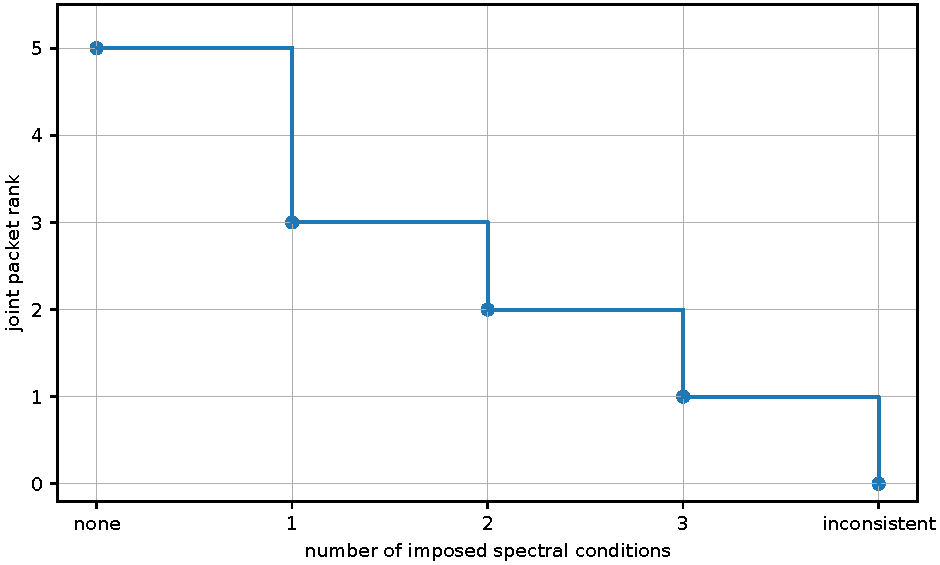
\includegraphics[width=.78\textwidth]{12_finite_occupancy.pdf}
\caption{Joint packet ranks descend as commuting conditions are imposed. In finite dimension, a positive rank sequence stabilizes.}
\label{fig:finite_occupancy}
\end{figure}

\section{Infinite occupancy and completion}\label{sec:infiniteoccupancy}

Finite stage nonvanishing does not always survive infinitely many conditions. The ambient compactness or finiteness hypothesis must be visible.

\begin{example}[Tail projection collapse]\label{ex:tail_projection}
Let \(H=\ell^2(\NN)\), with standard basis \((e_j)\). Let \(P_m\) be the orthogonal projection onto
\[
\overline{\operatorname{span}}\{e_m,e_{m+1},\ldots\}.
\]
Every range is nonzero and
\[
P_{m+1}P_m=P_{m+1}.
\]
Nevertheless,
\[
\boxed{
\bigcap_{m\geq1}\operatorname{ran}P_m
=\{0\}.
}
\]
\end{example}

\begin{proof}
A vector in every tail range has its first \(m-1\) coordinates equal to zero for every \(m\). Every coordinate is therefore zero.
\end{proof}

\begin{figure}[t]
\centering
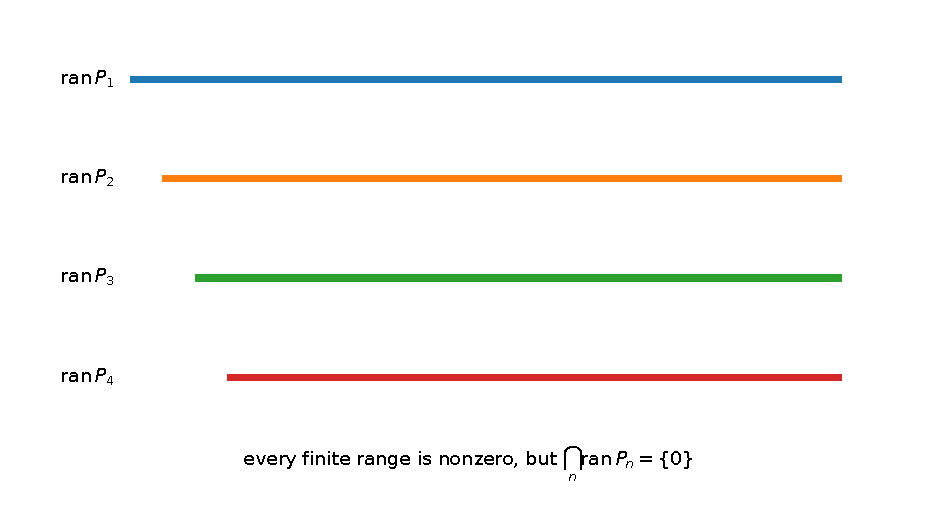
\includegraphics[width=.88\textwidth]{13_tail_projections.pdf}
\caption{Every finite tail is nonzero, while the infinite intersection is zero. Infinite dimensional occupancy needs an additional compactness or finiteness hypothesis.}
\label{fig:tail_projections}
\end{figure}

\begin{theorem}[Finite dimensional stabilization]\label{thm:finite_dim_stabilization}
Let
\[
V_1\supseteq V_2\supseteq V_3\supseteq\cdots
\]
be a descending chain of subspaces of a finite dimensional vector space. The chain stabilizes. If every \(V_m\) is nonzero, then
\[
\boxed{
\bigcap_mV_m\neq0.
}
\]
\end{theorem}

\begin{proof}
The dimensions form a nonincreasing sequence of nonnegative integers. Once the dimension stops decreasing, equality of dimensions and inclusion give equality of subspaces. A stabilized nonzero subspace is the intersection.
\end{proof}

\begin{theorem}[Finite length stabilization]\label{thm:finite_length_stabilization}
Let \(M\) be an Artinian module. Every descending chain of submodules stabilizes. If every member of the chain is nonzero, their intersection is nonzero.
\end{theorem}

\begin{proof}
The descending chain condition is the definition of an Artinian module. After stabilization, the intersection is the stable nonzero submodule.
\end{proof}

\begin{theorem}[Nested compact occupancy]\label{thm:nested_compact}
Let \(K_1\supseteq K_2\supseteq\cdots\) be nonempty closed subsets of a compact Hausdorff space. Then
\[
\boxed{
\bigcap_mK_m\neq\varnothing.
}
\]
\end{theorem}

\begin{proof}
The family has the finite intersection property because it is nested. Compactness gives a point in the total intersection.
\end{proof}

\begin{theorem}[Occupied inverse limit]\label{thm:occupied_inverse_limit}
Let \((Y_m)\) be an inverse system of finite nonempty sets satisfying the Mittag Leffler condition with nonempty stable cores. Then
\[
\varprojlim_mY_m
\neq
\varnothing.
\]
If every \(Y_m\) is a subset of a module quotient and excludes zero, every compatible branch is nonzero in every finite quotient.
\end{theorem}

\begin{proof}
The first statement is \cref{thm:finite_ml_branch}. The second is immediate from membership in each \(Y_m\).
\end{proof}

\subsection{Adic module completion}

\begin{standardfact}[Completion of finite modules]\label{fact:module_completion}
Let \(R\) be Noetherian, let \(I\subseteq R\), and suppose \(R\) is \(I\) adically complete. For every finite \(R\) module \(M\), the natural map
\[
M
\longrightarrow
\varprojlim_nM/I^nM
\]
is an isomorphism. The completion map \(R\to\widehat R\) is flat. See \cite{AtiyahMacdonald1969,Bourbaki1989,Matsumura1989}.
\end{standardfact}

\begin{theorem}[Formal occupancy reconstruction]\label{thm:formal_occupancy}
Let \(R\) and \(M\) satisfy \cref{fact:module_completion}. For each \(n\), let
\[
Y_n\subseteq M/I^nM
\]
be a finite nonempty set. Suppose the reduction maps carry \(Y_{n+1}\) into \(Y_n\), and the inverse system \((Y_n)\) satisfies the Mittag Leffler condition with nonempty stable cores. Then there is
\[
x\in M
\]
whose reduction belongs to \(Y_n\) for every \(n\). If zero belongs to none of the \(Y_n\), then \(x\neq0\).
\end{theorem}

\begin{proof}
Choose a compatible branch \((x_n)\in\varprojlim Y_n\) by \cref{thm:occupied_inverse_limit}. The completion isomorphism in \cref{fact:module_completion} gives a unique \(x\in M\) with these reductions. If \(x=0\), every reduction is zero, contrary to the hypothesis.
\end{proof}

\begin{corollary}[Surjective formal packet tower]\label{cor:surjective_formal_packet}
In \cref{thm:formal_occupancy}, it is enough to assume that every map
\[
Y_{n+1}\longrightarrow Y_n
\]
is surjective.
\end{corollary}

\begin{proof}
Surjectivity gives the Mittag Leffler condition with stable core \(Y_n\).
\end{proof}

\begin{theorem}[Support under adic completion]\label{thm:support_completion}
Let \(R\) be Noetherian, let \(I\subseteq R\), and let \(\widehat R\) be the \(I\) adic completion. For a finite \(R\) module \(M\),
\[
\boxed{
\Supp_{\widehat R}(M\otimes_R\widehat R)
=
\{\mathfrak q\in\Spec\widehat R:
\mathfrak q\cap R\in\Supp_R(M)\}.
}
\]
\end{theorem}

\begin{proof}
The completion map is flat. Apply \cref{thm:flat_base_change_support}.
\end{proof}

\begin{corollary}[Completion does not create support outside the original locus]\label{cor:completion_support_boundary}
Every occupied prime of the completed module lies above an occupied prime of the original module.
\end{corollary}

\begin{proof}
This is the inclusion contained in \cref{thm:support_completion}.
\end{proof}

\section{Conditional completion of an occupied system}\label{sec:completion}

The preceding theorems can be assembled once the required existence hypotheses are stated separately.

\begin{definition}[Declared arithmetic completion problem]\label{def:declared_completion_problem}
A declared completion problem consists of the following data.
\begin{enumerate}
\item A set of residual deformation functors at the coefficient places.
\item A common arithmetic spine \(\mathfrakC\).
\item Finite companion levels \(X_{\lambda,m}(\mathfrakC)\).
\item A compatible carrier or a finite module over a commutative carrier algebra.
\item A specified packet or support component whose nonvanishing is required.
\end{enumerate}
\end{definition}

\begin{theorem}[Conditional occupied system completion]\label{thm:conditional_completion}
Consider a declared arithmetic completion problem. Assume the following two completion hypotheses.

\begin{enumerate}
\item \textbf{Vertical completion.} For every coefficient place \(\lambda\), the natural map from the declared complete local realization space to
\[
\varprojlim_mX_{\lambda,m}(\mathfrakC)
\]
is a bijection, and the companion inverse system has nonempty stable core at every depth.
\item \textbf{Common spine.} Every finite companion level realizes the reduction of one fixed algebraic spine, and the local conditions are closed under inverse limits.
\end{enumerate}

Then there exists a simultaneous compatible family realizing the common spine.

Two further conclusions are available under separate occupancy hypotheses.

\begin{enumerate}
\item If the desired compatible constituents occur in a known carrier, are separated by finitely many Frobenius traces, and have a declared nonzero multiplicity vector satisfying the carrier capacity bounds, then the corresponding compatible summand occurs at every coefficient place. Its multiplicities are recovered from the finite trace separator.
\item If a finite module over a commutative carrier algebra is attached to the completed problem and its support meets a required component, then that component is occupied. The occupied locus is the vanishing set of the zeroth Fitting ideal.
\end{enumerate}
\end{theorem}

\begin{proof}
The vertical hypotheses and \cref{thm:one_place_completion} give a branch at every coefficient place. The common spine and \cref{thm:spine_recovery} identify the Frobenius data of the limiting branches. Simultaneous existence follows from \cref{thm:simultaneous_completion}.

Under the compatible carrier hypotheses, \cref{thm:frobenius_separation,thm:compatible_carrier} recover the declared nonzero multiplicity vector and transport the corresponding summand through the carrier. Under the module hypothesis, the required component meets \(\Supp_R(M)\), and \cref{thm:fitting_support} identifies this support with \(V(\Fitt_0^R(M))\). The two conclusions use different occupancy data and neither implies the other without an additional comparison theorem.
\end{proof}

\begin{corollary}[Exact remaining existence problems]\label{cor:remaining_problems}
The formal theorems do not supply either of the following statements.
\[
\boxed{
\begin{aligned}
&X_{\lambda,1}(\mathfrakC)\neq\varnothing
&&\text{for every required coefficient place }\lambda,\\
&\Supp_R(M)\cap C\neq\varnothing
&&\text{for every required global component }C.
\end{aligned}
}
\]
The first is companion existence. The second is occupancy or nonvanishing.
\end{corollary}

\begin{proof}
The branch theorems begin with nonempty stable cores. The support theorems detect an occupied locus but do not force a prescribed component to meet it.
\end{proof}

\begin{corollary}[Depth cannot repair a missing root]\label{cor:depth_cannot_repair}
Increasing the precision at occupied coefficient places cannot create a missing residual companion at another place.
\end{corollary}

\begin{proof}
Positive depth lifting stays inside one residual fiber by \cref{prop:no_crossing}. A missing companion means the required residual fiber is empty.
\end{proof}

\begin{corollary}[A projector cannot force occupancy]\label{cor:projector_cannot_force}
An exact spectral or central idempotent can measure the occupied submodule, but its existence does not imply that the corresponding component is nonzero.
\end{corollary}

\begin{proof}
The idempotent may act as zero. The trace and support criteria detect this case exactly.
\end{proof}

\begin{figure}[t]
\centering
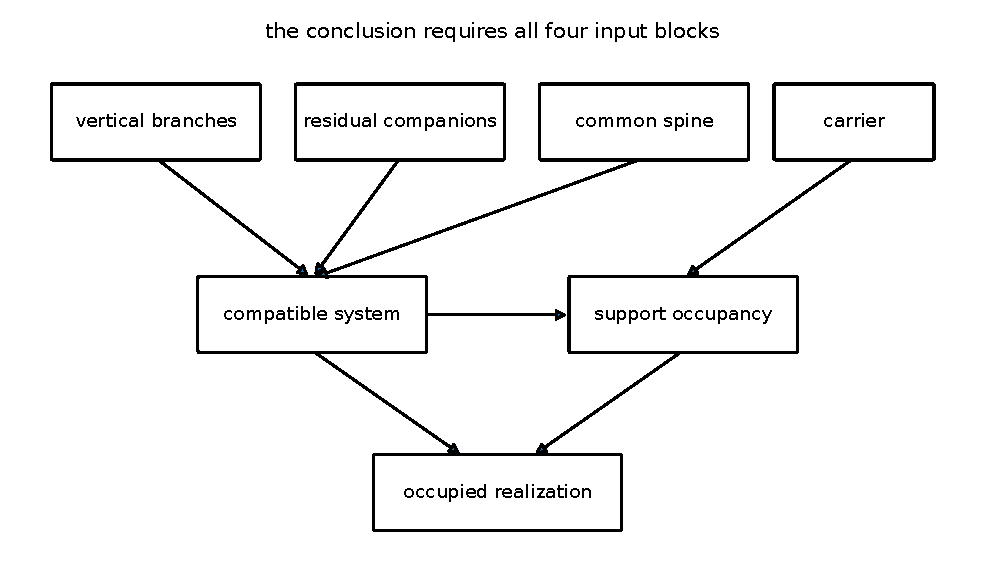
\includegraphics[width=.95\textwidth]{14_completion_dependencies.pdf}
\caption{The conditional conclusion requires vertical branches, residual companions, one common spine, and an occupied carrier component.}
\label{fig:completion_dependencies}
\end{figure}

\section{Examples and finite certificates}\label{sec:examples}

The examples in this section are small exact models. They test the formulas and expose failure modes. They do not replace deformation theory or arithmetic existence theorems.

\subsection{A smooth branch}

Take \(q=3\) and relative dimension \(d=2\). The first levels have cardinalities
\[
1,9,81,729,6561.
\]
The level series is
\[
Z(T)=\frac{T}{1-9T}.
\]

\subsection{A weighted dyadic branch}

For weights \((1,2,4)\), the first counts are
\[
1,2,8,32,256,2048.
\]
The first coordinate appears immediately, the second appears after one delay, and the third appears after three further levels. The level series is
\[
Z(T)
=
T+2T^2+8T^3+32T^4+
\frac{256T^5}{1-8T}.
\]

\subsection{A square nilpotent branch}

For \(x^2=0\) over a residue field of size three, the level counts are
\[
1,3,3,9,9,27,27,81.
\]
The series is
\[
Z(T)=\frac{T+3T^2}{1-3T^2},
\]
and the branching exponent is \(1/2\).

\subsection{A normal crossing branch}

For \(xy=0\) over the same residue field, the first counts are
\[
5,21,81,297,1053.
\]
The additional factor linear in the depth distinguishes the crossing from a smooth one dimensional branch, even though both have branching exponent one.

\subsection{Finite Frobenius recovery}

Use the trace matrix
\[
C=
\begin{pmatrix}
1&1&1\\
1&2&3\\
3&0&1
\end{pmatrix}
\]
and multiplicity vector
\[
\bm m=(2,0,1)^T.
\]
The observed trace vector is
\[
C\bm m=(3,5,7)^T.
\]
The determinant of \(C\) is nonzero, so the multiplicities are recovered uniquely.

\subsection{Finite occupancy}

A sequence of commuting projectors with ranks
\[
3,2,1,0
\]
shows both outcomes. The first three conditions leave one occupied joint packet. The final inconsistent condition makes the packet empty.

\section{Logical boundaries}\label{sec:boundaries}

\begin{longtable}{>{\raggedright\arraybackslash}p{.31\textwidth}>{\raggedright\arraybackslash}p{.21\textwidth}>{\raggedright\arraybackslash}p{.39\textwidth}}
\caption{Status of the principal result blocks.}\label{tab:status}\\
\toprule
Block & Status & Boundary\\
\midrule
\endfirsthead
\toprule
Block & Status & Boundary\\
\midrule
\endhead
Residual partition & Proved & Requires a declared reduction map\\
Inverse limit reconstruction & Proved & Requires completeness or a stable finite inverse system\\
Smooth and weighted counts & Proved & Applies only after the local chart is established\\
Nilpotent and crossing counts & Proved & These are explicit model singularities\\
Cohomology packet splitting & Proved & Projectors must commute with the differential\\
Packet lifting criterion & Proved & Requires a complete declared obstruction theory\\
Directed source count & Proved & Counts generation among existing roots only\\
Companion completion & Proved conditionally & Every local stable core must be nonempty\\
Finite Frobenius separation & Proved & Constituents must be pairwise nonisomorphic at one place\\
Compatible carrier propagation & Proved conditionally & A compatible carrier decomposition must already be known\\
Fitting support occupancy & Proved & Detects support but does not force a chosen component to occur\\
Finite joint trace criterion & Proved & Applies in a fixed finite carrier\\
Infinite nonvanishing & Proved under stated compactness conditions & Finite stage nonvanishing alone is insufficient\\
Universal residual companions & Not proved & Requires arithmetic existence at every coefficient place\\
Universal global occupancy & Not proved & Requires nonvanishing on the desired global component\\
Unrestricted reciprocity & Not claimed & Needs local and global realization theorems beyond this article\\
\bottomrule
\end{longtable}

\subsection{Historical scope}

The residual and obstruction theory used here rests on established deformation theory \cite{Schlessinger1968,Mazur1989,Ramakrishna1993,Kisin2010}. Compatible systems and Frobenius comparison are classical themes in \cite{Serre1998,LarsenPink1992,BellaicheChenevier2009}. The support and Fitting ideal results are standard commutative algebra \cite{AtiyahMacdonald1969,Eisenbud1995,Matsumura1989}. The contribution of the article is the exact assembly of these layers with explicit finite counting, transport, and nonvanishing criteria. No theorem is assigned historical priority without a separate comparison with the specialized literature.

\section{Conclusion}\label{sec:conclusion}

A residual deformation problem begins with a disjoint special fiber. Each residual point supports its own lift forest. Completeness reconstructs a branch from compatible finite levels, while the Mittag Leffler condition identifies the stable part of a forest when some finite nodes die. Weighted visibility and singular level counts record how the local geometry appears with increasing precision.

Tangent and obstruction spaces split when the correction complex has compatible projectors. This gives a precise packet criterion for lifting. Horizontal transport then acts between residual roots. Its source components count the number of starting roots required to generate a finite transport graph, but the graph cannot create a root that is absent.

Compatible systems require one algebraic spine and one occupied companion branch at every coefficient place. Finite Frobenius traces recover compatible multiplicities once the desired constituent sits inside a known carrier. Support theory supplies the correct nonsemisimple occupancy language. The zeroth Fitting ideal detects whether a component is present, and adic completion preserves support by flat base change.

The remaining arithmetic problems are therefore explicit. One must prove that every required residual companion exists and that the intended global component is occupied. Vertical depth, formal projectors, and finite trace formulas organize these problems. They do not solve the missing existence statements by themselves.

\section*{Language model contribution}

An OpenAI language model was used as an organizational and mathematical drafting aid. Its contributions included suggestions for the Mittag Leffler formulation in \cref{sec:residual}, the visibility and singular count expansions in \cref{sec:counting}, the support and Fitting ideal organization in \cref{sec:support}, the finite and infinite occupancy distinction in \cref{sec:finiteoccupancy,sec:infiniteoccupancy}, and the grouping of hypotheses in \cref{sec:completion}. The author assumes full responsibility for independently verifying every statement, proof, calculation, and reference in any submitted version. The model is not an author.

\bibliographystyle{amsplain}
\bibliography{PSC_Paper_X_Strengthened_Annals_Edition}

\end{document}
